\chapter{Motivation}\label{chap:motivation}

\begin{figure}
    \centering
    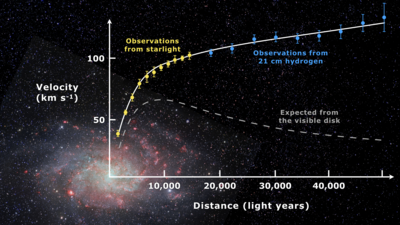
\includegraphics[width=0.85\textwidth]{figs/motivation/dm.png}
    %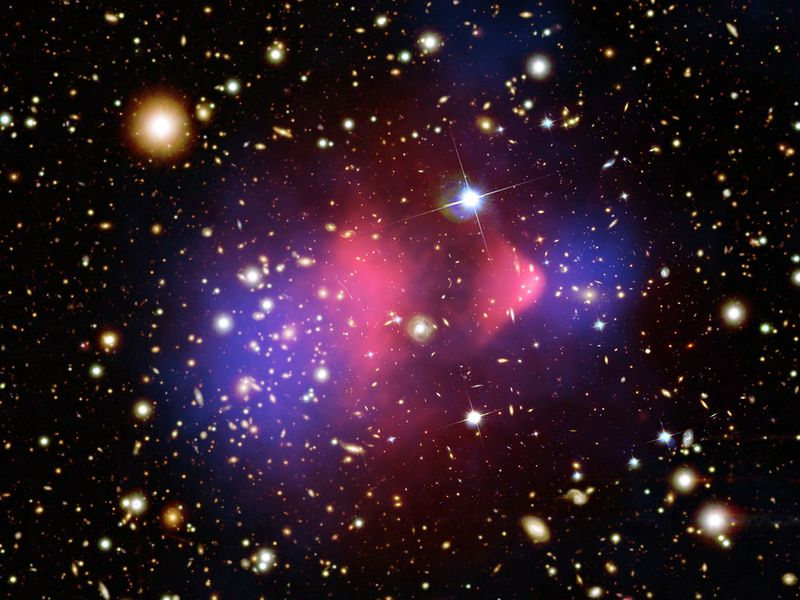
\includegraphics[width=0.6\textwidth]{figs/motivation/bulletcluster.jpg}
    %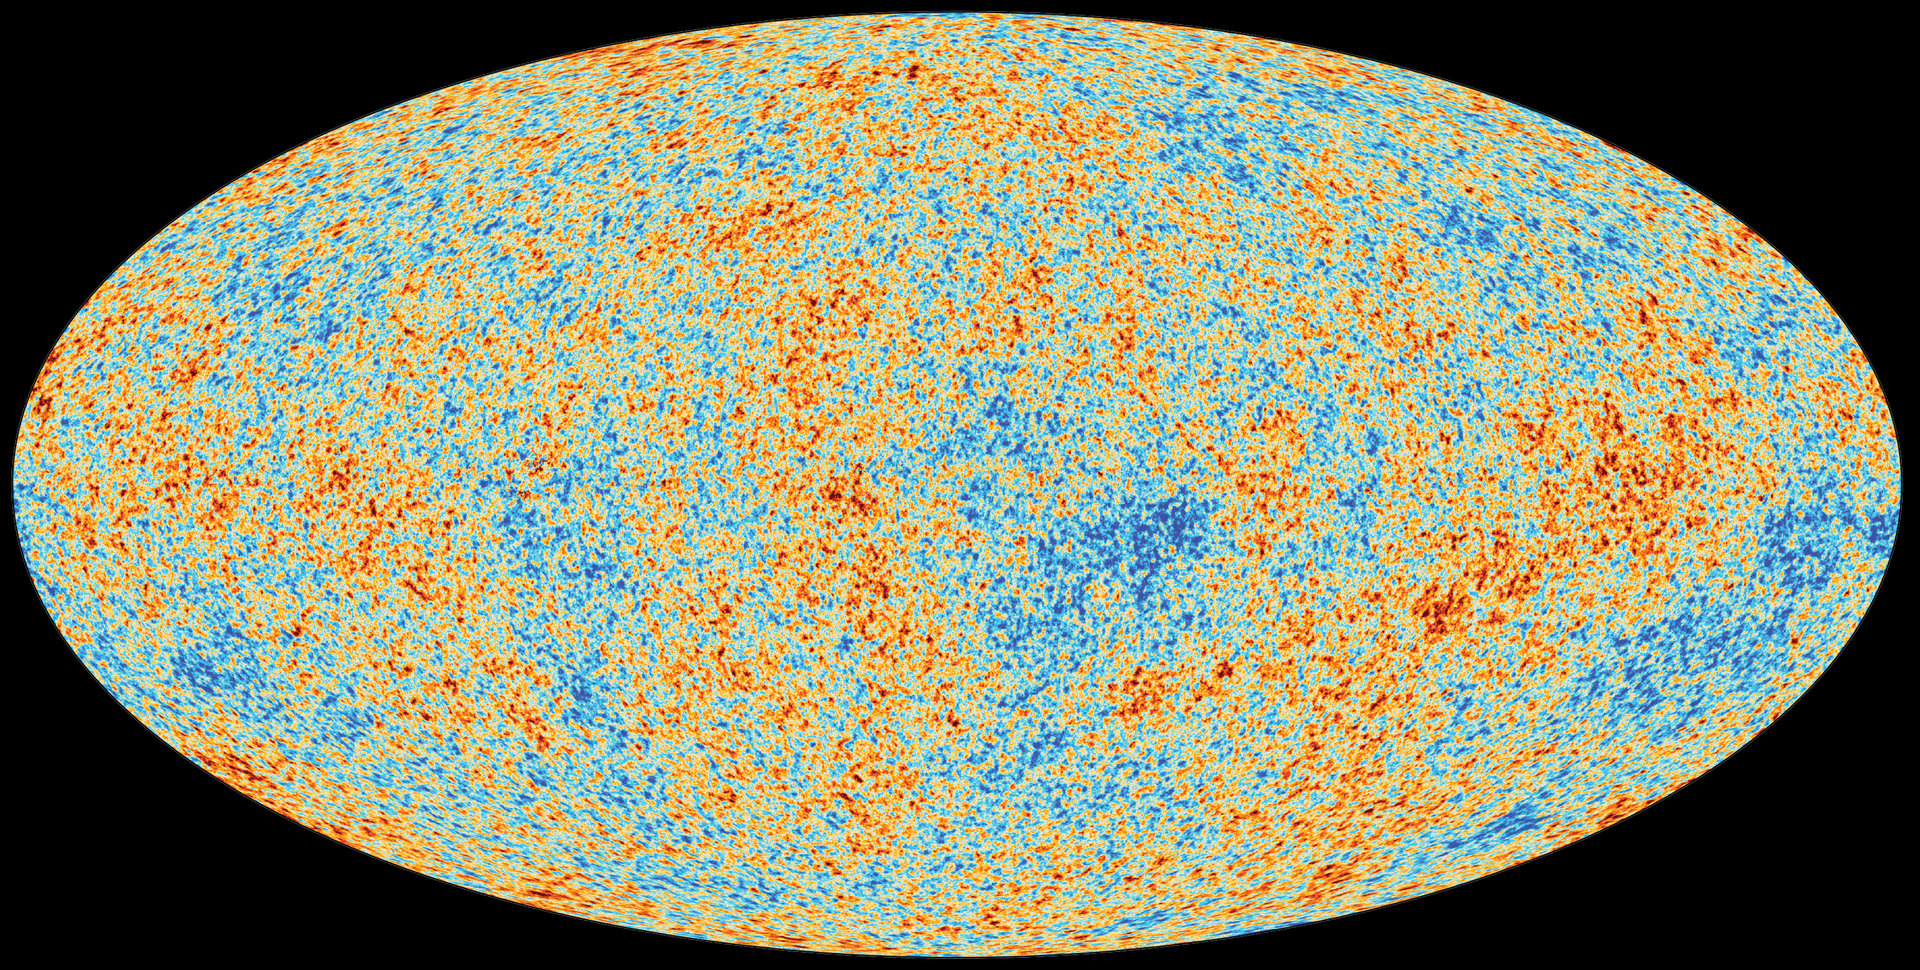
\includegraphics[width=0.6\textwidth]{figs/motivation/cmb.jpg}
    \caption{Galactic rotation curves show stars far from the galactic center are orbiting the galactic center far faster than they should gives evidence for invisible matter.}
    \label{fig:rotationcurve}
\end{figure}

The Standard Model of Particle Physics (SM) has remained the best description of elementary particles and their interactions since its formulation. However, there are several observations, particularly measurements from cosmology, that show that the Standard Model is incomplete. %description of the universe shown in Fig.~\ref{fig:sm} is incomplete.

\section{Observations}\label{sec:observations}

The modern evidence for invisible matter beyond the SM stems mainly from galactic rotation curves, weak gravitational lensing, the cosmic microwave background (CMB), big bang nucleosynthesis (BBN), and Type 1a supernovae.

\subsection{Galactic Rotation Curves}\label{sec:galactic}

The first modern evidence for invisible matter comes from Vera Rubin's measurements of galactic rotation curves (i.e. the velocity at which stars orbit their galactic center) in the 1970s. Based on kinematics and the gravitational inverse square law, in the absence of invisible matter, one expects the speed at which stars orbit their galactic center to scale with the the distance from the center $r$ as $1/\sqrt{r}$. However, Vera Rubin's measurements show that these velocities were flat with increasing $r$ even for stars far away from the galactic center \cite{Rubin:1980zd}. This discrepancy between theory and measurements can be explained by the presence of matter that cannot be visibly detected. This effect is shown in Fig. \ref{fig:rotationcurve}.

\clearpage

\subsection{Weak Gravitational Lensing}\label{sec:gravitationallensing}

\begin{figure}
    \centering
    %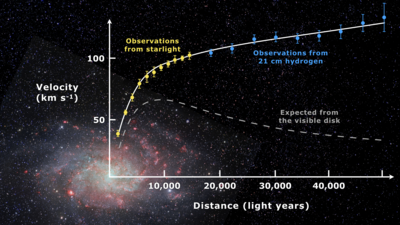
\includegraphics[width=0.6\textwidth]{figs/motivation/dm.png}
    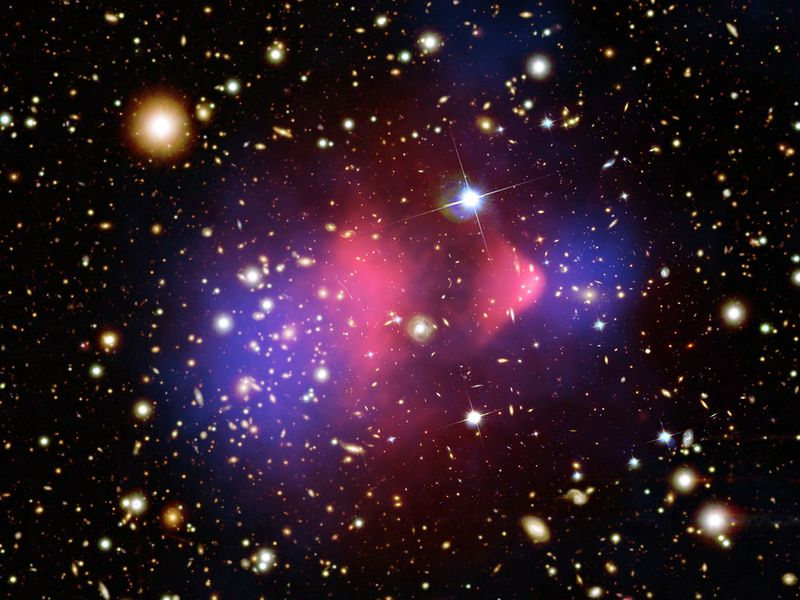
\includegraphics[width=0.85\textwidth]{figs/motivation/bulletcluster.jpg}
    %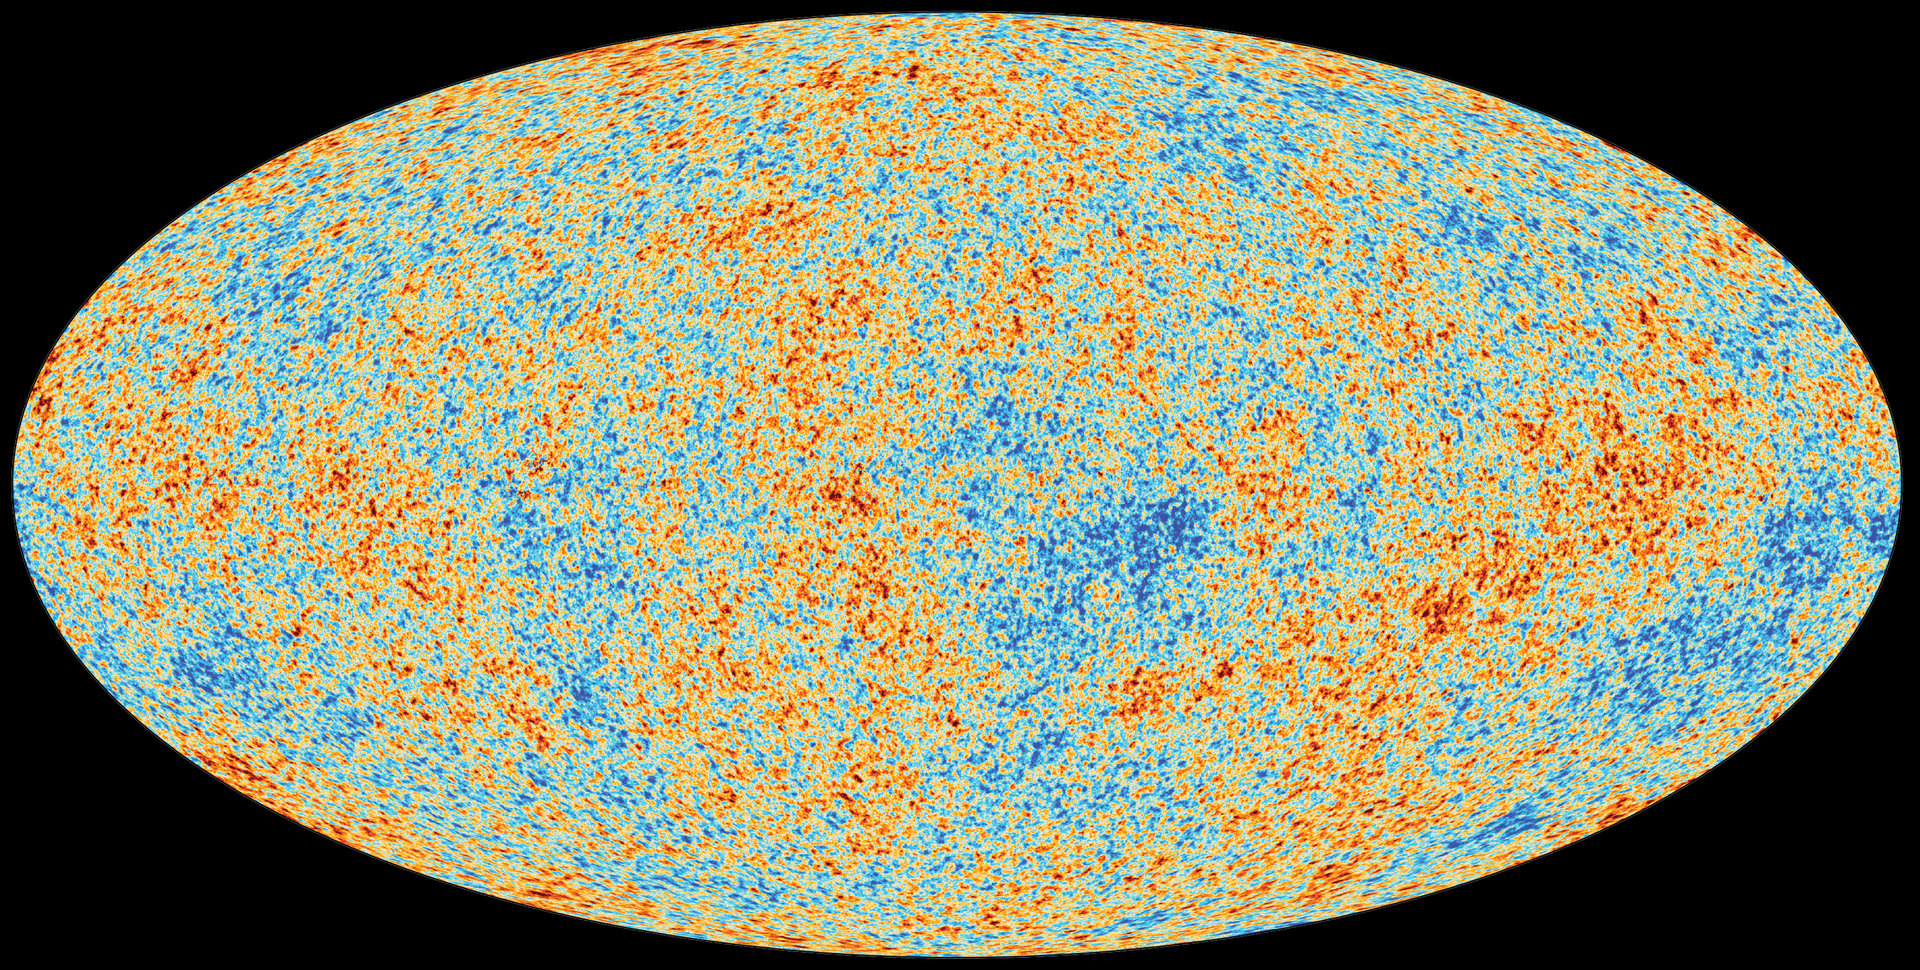
\includegraphics[width=0.6\textwidth]{figs/motivation/cmb.jpg}
    \caption{The Bullet Cluster shows visible matter from X-rays (highlighted in blue) and total matter from gravitational lensing (highlighted in pink). The distribution of visible matter and total matter is not in agreement.}
    \label{fig:lensing}
\end{figure}

One could suppose that, since no independent tests of gravity are applied at the galactic scale, gravity could simply be poorly understood at this scale. This is a possibility, in fact throughout the history of astronomy, there is often the tension between a new theory of gravity and the presence of some form of unseen matter as a resolution to an anomaly. %The former won in cases such as heliocentricity in favor of geocentricity describing the effect of ``epicycles'' during the times of Copernicus and the orbit of Mercury being explained by Einstein's General Relativity as opposed to Newton's theory of universal gravitation. The latter won in the case with the discovery of Uranus. Though various theories of modified gravity such as Modified Newtonian Dynamics (MoND) or TEVAS successfully resolve the problem of galactic rotation curves, it fails to account for observations from weak gravitation lensing.

However, in addition to galactic rotation curves, measurements from gravitational lensing - the bending of light in the presence of matter - provide evidence for invisible matter that cannot be accounted for by the SM. The measurement of the bending of light originating from distant galaxies provides a measurement of the total mass in large regions of galactic clusters. This can be compared with the distribution of X-rays from colliding galactic clusters, which is thought to be proportional to the distribution of visible matter in the galactic cluster. In a measurement of two colliding galactic clusters known as the Bullet Cluster shown in Fig. \ref{fig:lensing}, the distribution of visible matter from X-ray measurements (reconstructed in pink) does not agree with the distribution of the total amount of matter as inferred from weak gravitational lensing (reconstructed in blue) \cite{Clowe_2004}. This is clear indication that there is invisible matter located within the Bullet Cluster that is non-baryonic and cannot be accounted for by a different theory of gravity.

\clearpage

%\subsection{Cosmic Microwave Background}\label{sec:cmb}
\subsection{Baryon Acoustic Oscillations}\label{sec:cmb}

\begin{figure}
    \centering
    %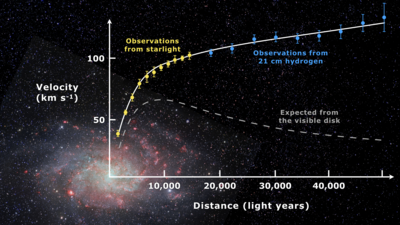
\includegraphics[width=0.6\textwidth]{figs/motivation/dm.png}
    %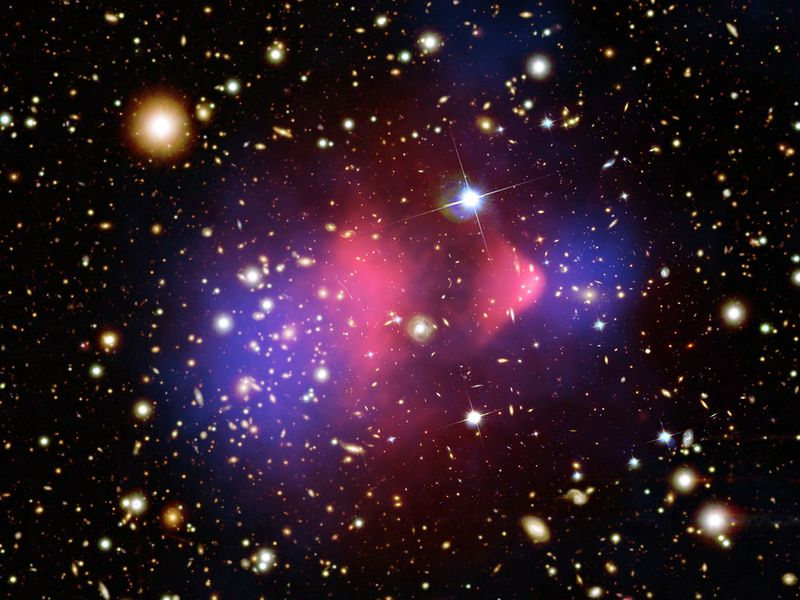
\includegraphics[width=0.6\textwidth]{figs/motivation/bulletcluster.jpg}
    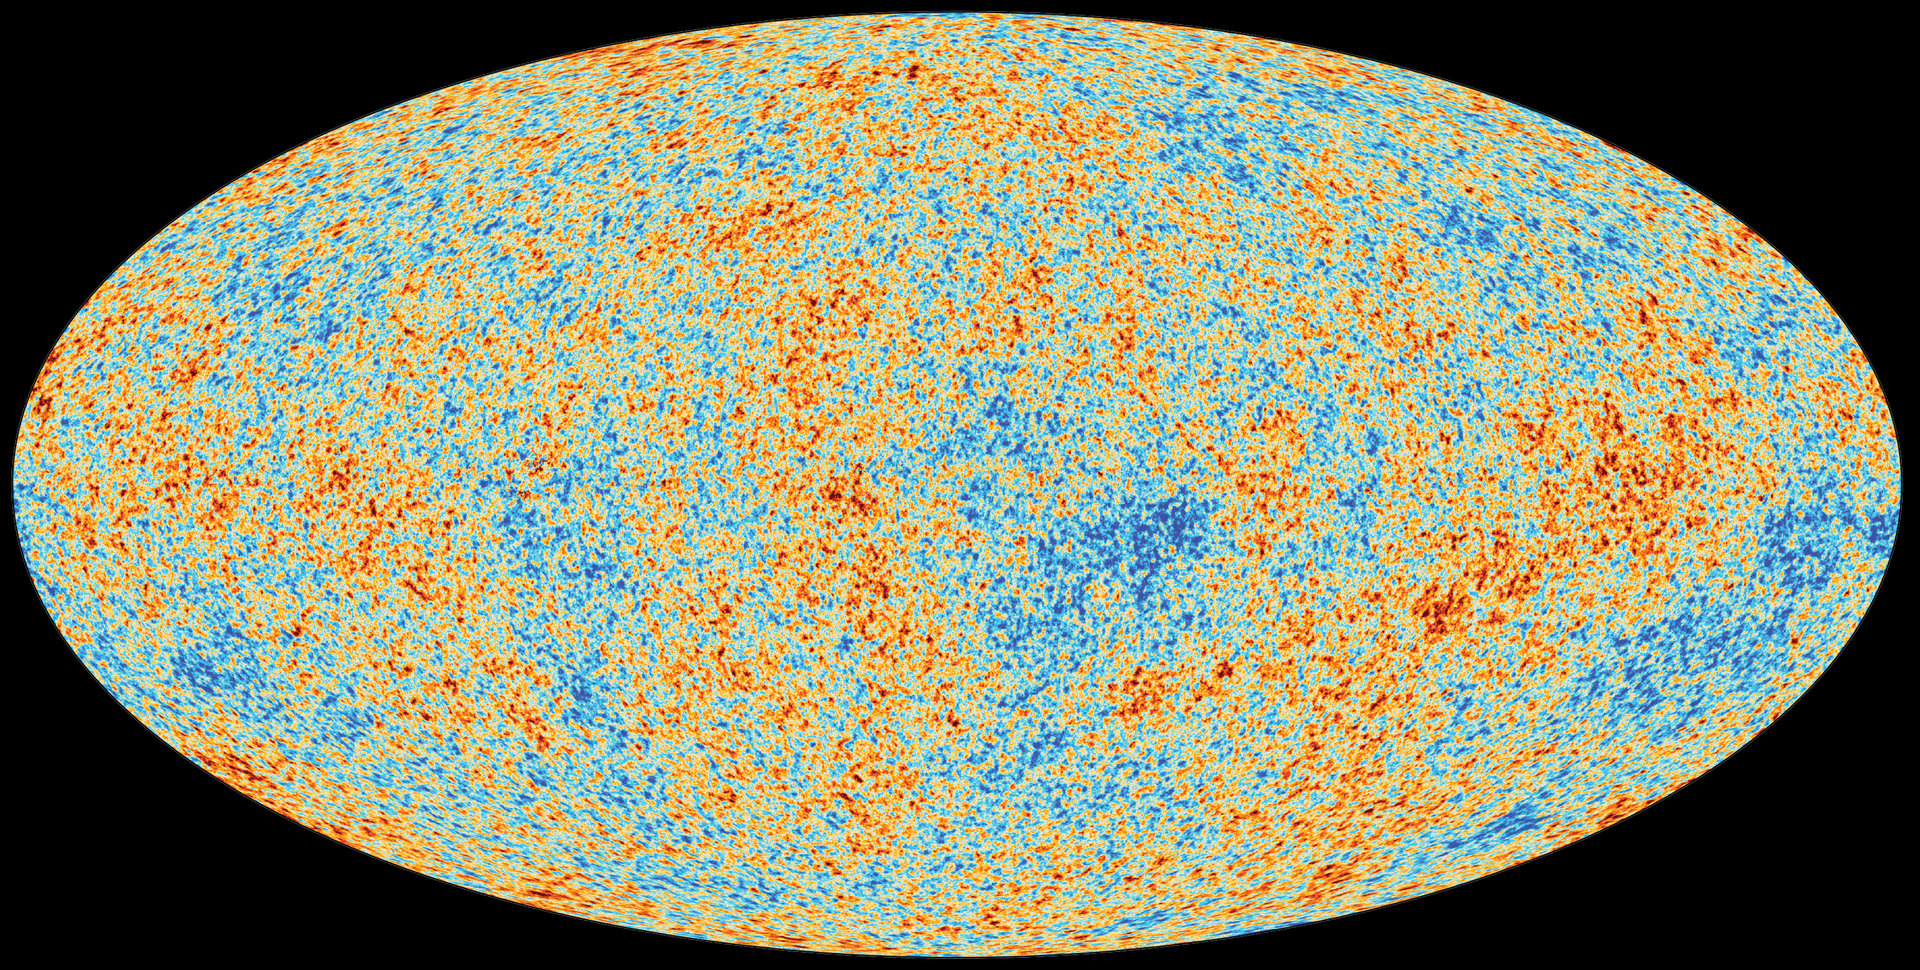
\includegraphics[width=0.85\textwidth]{figs/motivation/cmb.jpg}
    \caption{The Cosmic Microwave Background has temperature fluctuations which can be correlated to measure the propagation of sound waves in the early universe. This propagation is consistent with extra invisible matter in the early universe.}
    \label{fig:dm}
\end{figure}

The existence of invisible matter, or dark matter, is supported by the anomalies of both galactic rotation curves and gravitational lensing. However, these evidences alone do not rule out the possibility of a SM explanation of this invisible matter, or establish it being particulate in nature at all. For instance, black holes are a possible form of a non-particulate invisible matter that involve neither new particles beyond the SM or a particle nature of dark matter. Despite this, there are several other pieces of evidence that extend the case for dark matter.

In the early universe, acoustic density waves caused fluctuations in the density of baryonic matter in the primordial plasma. This phenomenon is called the baryon acoustic oscillations (BAO) and provides a ``standard ruler'' for a cosmological length scale ($\sim$490 million light years in today's universe). Acoustic density waves are caused by the simultaneous counteraction of the gravitational pull of all matter and the pressure exerted outward by baryonic matter in over dense regions. Dark matter stays at the center of these over dense regions in the center of the acoustic density waves while baryonic matter and photons propagate outwards until decoupling when photons no longer interact with matter. 

%The speed, amplitude, and wavelength are determined by the amount of baryonic matter and the total amount of matter (i.e. baryonic and dark matter) and a measurement of these properties of the wave provide these measurements. 

The over and under dense regions of the primordial plasma cause temperature fluctuations that can be measured in the cosmic microwave background (CMB) anisotropies, the thermal ``afterglow'' of the Hot Big Bang at the time of decoupling. Thus, a measure of the size of the over densities as well the standard size of the oscillations embedded in the power spectrum of the CMB anisotropies provides a direct measurement of baryonic matter and total matter. %through the correlations in the temperature fluctuations in the CMB spectrum (where over dense regions correspond to hotter regions), called CMB anisotropies shown in \ref{fig:dm}... The BAO provides a quantitative measurement of both the amount of total matter and the amount of baryonic matter in the early universe. 
Of the total matter in the early universe, precision BAO measurements gives about $\sim$15\% baryonic matter (which is representative of the total SM matter in the early universe) and 85\% of an additional type of matter. This matter discrepancy is in agreement with the anomalies described by the galactic rotation curves and gravitational lensing suggesting that the same invisible matter that is observed in the universe today is the same type of invisible matter that existed in the early universe. The measurement of the BAO from the CMB is also in excellent agreement with measurements of large scale structure in which galaxies at the standard cosmological distance are correlated as one would expect if these over dense regions in the early universe formed galaxies in a bottom up fashion.

%The cosmic microwave background (CMB), the thermal ``afterglow'' of the Hot Big Bang, shows evidence for invisible matter in the early universe that cannot be explained by the SM shown in the bottom of Fig. \ref{fig:dm}. Specifically, the correlations in the temperature fluctuations in the CMB spectrum, called CMB anisotropies, provide a measurement of sound waves in the early universe (called baryon acoustic oscillations, or simple BAO). This provides a quantitative measurement of both the amount of total matter and the amount of baryonic matter in the early universe. Of the total matter in the early universe, precision BAO measurements gives about $\sim$15\% baryonic matter (which is representative of the total SM matter in the early universe) and 85\% of an additional type of matter. This matter discrepancy is in agreement with the anomalies described by the galactic rotation curves and gravitational lensing suggesting that the same invisible matter that is observed in the universe today is the same type of invisible matter that existed in the early universe. \textcolor{red}{John says I lump BAO and CMB together. I always thought these were one in the same. If not, I could use some guidance for their distinction.}

This does not explicitly rule out the possibility that dark matter consists of primordial black holes, that is those that existed and were formed in the early universe. However, primordial black holes as an explanation of dark matter are tightly constrained and thus are not favored \cite{carr2020constraints}.  %because they require unnatural fine tuning to get the models to produce observed results are do not explain the next anomaly - the upper bound on baryonic matter set by Big Bang Nucleosynthesis.

\clearpage

\subsection{Big Bang Nucleosynthesis and Type 1a Supernovae}\label{sec:bbn}

Measurements from Type 1a Supernovae, known as a ``standard candle'' because of their well-defined and easily identifiable light curves that have a known and essentially fixed luminosity (so a measurement of its brightness tells its distance), provide a measurement of the total matter in the universe. In the framework of the $\Lambda$CDM Model, a comparison of the redshift and luminosity of these supernovae gives a measurement of 30\% matter of the total energy budget of the universe which is in agreement with CMB measurements \cite{Amanullah_2010}.\footnote{The $\Lambda$CDM Model (dark energy and cold dark matter) is the standard model of cosmology built on the framework of General Relativity. Dark energy is the energy responsible for the accelerated expansion of the universe as measured by the Type 1a Supernovae and CMB. The fundamental nature and origin of dark energy is also a mystery and will not be discussed further.}

On the other hand, Big Bang Nucleosynthesis (BBN), the description of production of hydrogen, deuterium, helium, and lithium nuclei in the early universe, constrains the current observed density of these nuclei with the primordial nucleon density. The observed density of all these nuclei are in agreement if the relative density of primordial baryonic matter in the universe is $<\sim5$\% ($\Omega_b< \sim 0.05$) \cite{1998RvMP...70..303S}. This is far below the total mass measurement from Type 1a Supernovae at 30\% suggesting much of matter in the universe is non-baryonic, and hence beyond the SM. The measurements from Type 1a Supernovae and BBN are shown in Fig. \ref{fig:bbn}

%Quantitatively, all this evidence shows that the dark matter makes up about 85\% of the total mass in the universe (about 25\% of the total energy budget of the universe, much of the remainder is due to dark energy). Particularly, the galactic rotation curves and the CMB evidence shows that the same dark matter that is around today was the same dark matter around in the early universe. This gives a strong hint that dark matter has a thermal origin, meaning it was in thermal equilibrium with Standard Model matter in the early universe until ``Freeze Out'', the point at which the amount of dark matter is set in the universe.

\begin{figure}
    \centering
    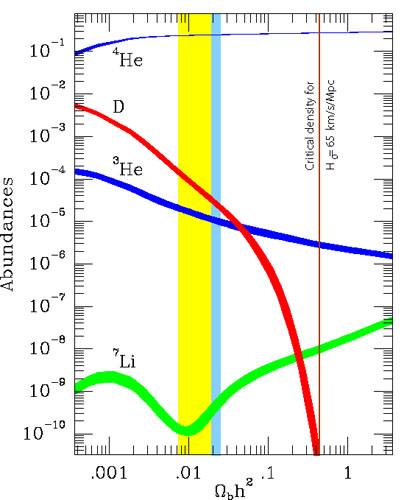
\includegraphics[width=0.44\textwidth]{figs/motivation/bbn.jpg}
    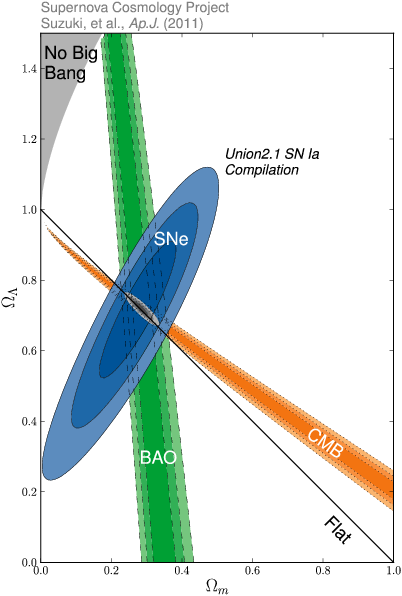
\includegraphics[width=0.36\textwidth]{figs/motivation/scp.png}
    \caption{Left: Big Bang Nucleosynthesis puts an upper bound on the Standard Model matter density in the universe at about 15\% of the total matter budget \cite{1998RvMP...70..303S}. Right: Measurements from Type 1a supernovae (shaded in blue) together with the CMB and BAO measurements put the total mass in the universe at 30\% of the total energy budget along with dark energy at 70\% (from the intersection in gray) \cite{Amanullah_2010}. A combination of these measurements show that the Standard Model cannot account for most of the matter in the universe.}
    \label{fig:bbn}
\end{figure}

\subsection{Some Properties of Dark Matter}\label{sec:properties}

From these measurements, one can constrain the properties of this missing matter. Any potential explanation of this missing matter must account for the following. 

\begin{enumerate}
  \item Since it has evaded all detection mechanisms other than gravitational effects thus far, this missing matter is invisible and does not interact appreciably with SM photons. Hence, the common term for this matter is ``dark matter.''
  \item Measurements of the amount of dark matter from the early universe, particularly from the CMB, agree with present measurements. This indicates that dark matter is stable with a livetime far greater than the 13.8 billion year age of the universe.
  \item Measurements from different regions of the universe are consistent with the idea of missing matter. This, together with the Cosmological Principle, provides compelling evidence that dark matter is present everywhere in the universe, including here on Earth.
  \item The density of dark matter in the universe is similar to the density of SM matter (i.e. they have the same order of magnitude). A natural explanation for this coincidence is that there is some interaction, even indirect, between dark matter and SM matter in the early universe that connects their origins. This is the basis for the concept of ``thermal dark matter'' in which dark matter and SM matter were in thermal equilibrium until the universe cooled to the $\sim$MeV scale (which is the temperature scale that Big Bang Nucleosynthesis occurred).
\end{enumerate}

These measurements, specifically the CMB and Type 1a Supernovae measurements, together with the $\Lambda$CDM Model also provide a quantitative breakdown of the energy budget of the universe. Matter itself only composes about 30\% ($\Omega_m=30$\%) of the energy budget. The remaining 70\% is due to dark energy ($\Omega_{\Lambda}=70$\%). Within the matter budget, dark matter comprises about 85\% of the total mass ($\Omega_{DM}=26$\%) while SM matter, which includes our everyday atoms and molecules, comprises only 15\% of the total mass in the universe ($\Omega_{SM}=4$\%). Furthermore, any model of dark matter must respect this observed value of $\Omega_{DM}$ called the ``relic density'' (any model that overproduces dark matter can be immediately ruled out).

\clearpage

%\section{Dark Matter Thermal Freeze Out}\label{sec:freezeout}

%The galactic rotation curves and the CMB evidence shows that the same dark matter that is around today was the same dark matter around in the early universe. In addition, they are about the same... This gives motivation for a thermal origin of dark matter meaning that it was in thermal equilibrium in the early universe with Standard Model particles. One method of thermal dark matter, called thermal freezeout, is annihilation... This mechanism is illustrated in Fig. \ref{fig:freezeout}.

%Additional fundamental forces gives rise to...

%\begin{figure}
%    \centering
%    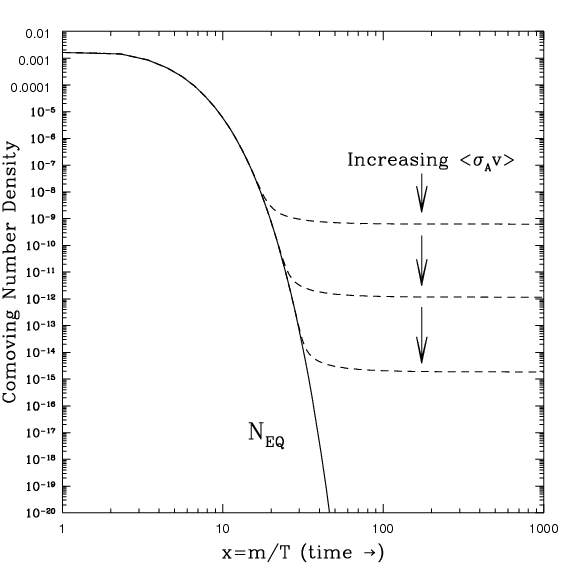
\includegraphics[width=0.5\textwidth]{figs/motivation/thermalfreezeout.png}
%    \caption{Thermal Freezeout}
%    \label{fig:freezeout}
%\end{figure}

\section{Theory Summary}\label{sec:theory}

\begin{figure}
    \centering
    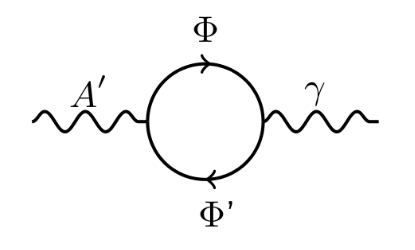
\includegraphics[width=0.5\textwidth]{figs/motivation/oneloop.png}
    \caption{A one-loop kinetic mixing process where an $\aprime$ mixes with the SM photon through an interaction of massive fields that couple to both photons.}
    \label{fig:km}
\end{figure}

Heavy photons appear in a variety of dark matter scenarios typically acting as a mediator between dark matter particles as well as providing indirect interactions with SM matter, and detailed motivations for dark matter with a heavy photon hypothesis will be described in detail in Sec. \ref{sec:history} and Sec. \ref{sec:ldm}. But first, it is important to understand the basics of heavy photon formalism.

A theory that has gained interest over the past few years is that of an additional Abelian gauge symmetry $U'(1)$. The additional symmetry was first proposed by Holdom in 1985 and is the basic assumption behind the existence of a heavy photon where the additional broken symmetry interacts with the SM hypercharge via kinetic mixing \cite{Holdom:1985ag}. Suppose nature does contain this additional Abelian gauge symmetry $U'(1)$ which contains a massive gauge boson $\aprime$. This would produce the following Lagrangian:

%\footnote{The original proposal of broken symmetry was proposed as a Stukelberg mechanism.} 

\begin{equation}
    \mathcal{L} = \mathcal{L}_{SM} + \frac{1}{4} F'^{\mu\nu}F'_{\mu\nu} + m^2_{\aprime} A'^{\mu}A'_{\mu} + \epsilon F^{\mu\nu}F'_{\mu\nu}
    \label{eqn:lagrangian}
\end{equation}

where $\mathcal{L}_{SM}$ is the Standard Model Lagrangian, $F_{\mu\nu}$ is the electromagnetic field strength, $F'_{\mu\nu} = \partial_{\mu}A'_{\nu} - \partial_{\nu}A'_{\mu}$ is the heavy photon field strength tensor (SM hypercharge), and $\epsilon$ is a dimensionless coupling constant also called the kinetic mixing parameter. This additional symmetry gives rise to a kinetic mixing term $\epsilon F^{\mu\nu}F'_{\mu\nu}$ with $\epsilon$ as the kinetic mixing parameter where the Standard Model photon mixes with the a new gauge boson, an $\aprime$, through an interactions of massive fields $M_{\Phi}$ and $M_{\Phi '}$ as shown in Fig \ref{fig:km}. These intermediate particles could be massive far above the Supersymmetry-breaking scale, but the kinetic mixing will persist down to much lower mass scales. Due to kinetic mixing, the fields are non-orthogonal, but orthogonality can be restored by redefining the electromagnetic field as $A^{\mu} \rightarrow A^{\mu}+ \epsilon A'^{\mu}$. By removing all the resulting $\epsilon^2$ terms, this diagonalizes the gauge terms in the Lagrangian in Eq. \ref{eqn:lagrangian} as

\begin{equation}
    \mathcal{L}_{gauge} = - \frac{1}{4} F'^{\mu\nu}F'_{\mu\nu} - \frac{1}{4} F^{\mu\nu}F_{\mu\nu}
    \label{eqn:gauge}
\end{equation}

The redefinition of the gauge field also changes the interaction term of the Lagrangian $\mathcal{L}_{int}=A^{\mu} J_{\mu}^{EM}$ to 

\begin{equation}
    A^{\mu} J_{\mu}^{EM} \rightarrow (A^{\mu}+\epsilon A'^{\mu}) J_{\mu}^{EM}
    \label{eqn:interaction}
\end{equation}

This induces an effective coupling between the heavy photon field and the electromagnetic current that is proportional to a factor $\epsilon$. Perturbativity requires $\epsilon<1$, thus $\epsilon$ suppresses the effective charge. One loop processes such as the one shown in Fig. \ref{fig:km} can be naturally generated by heavy multiplets that are charged under both the SM electric charge and a dark charge (the charge resulting from the new symmetry) \cite{ArkaniHamed:2008qp} \cite{Bjorken:2009mm}. This process motivates $\epsilon$ to be in the range $\sim 10^{-2}-10^{-4}$ and can be related to several parameters by the following:

%This additional symmetry gives rise to a kinetic mixing term $\epsilon F^{\mu\nu}F'_{\mu\nu}$ with $\epsilon$ as the kinetic mixing parameter where the Standard Model photon mixes with the a new gauge boson, an $\aprime$, through an interactions of massive fields $M_{\Phi}$. This induces an indirect coupling $\epsilon e$ of an $\aprime$ to Standard Model fermions. This is also known as a ``vector portal'' as this provides an indirect way that Standard Model particles can interact with hidden sector particles, which don't interact with Standard Model particles by definition. For one loop processes shown in Fig. ??, the kinetic mixing parameter is motivated to be

\begin{equation}
    %\epsilon \sim \frac{e g_D}{16 \pi^2} \ log \left( \frac{M_{\Phi}}{\Lambda} \right) \sim  10^{-2} - 10^{-4}
    \epsilon \sim \frac{e g_D}{16 \pi^2} \ log \left( \frac{M_{\Phi}}{M_{\Phi '}} \right) \sim  10^{-2} - 10^{-4}
    \label{eqn:epsilon}
\end{equation}
where $e$ is the electric charge and $g_D$ is the hypercharge dark coupling. %, and $\Lambda$ is some cutoff value.
If the theory does not contain these additional particles that are charged under both $U(1)$ symmetries, additional loop processes are possible and motivated by Grand Unification Theories (GUT) generally in the range $\epsilon \sim 10^{-3}-10^{-6}$ \cite{ArkaniHamed:2008qp}. Finally, some versions of string theory motivate $\epsilon$ below $10^{-6}$ \cite{Goodsell:2010ie} \cite{Goodsell:2009xc} \cite{Cicoli:2011yh} \cite{Jaeckel_2010}. Models of light dark matter, where the dark matter mass is below the Lee-Wienberg bound as described in Sec. \ref{sec:ldm}, as well as certain models of supersymmetry motivate mass scales of MeV-GeV. String theories connect $\epsilon$ to the mass scale resulting in a motivated mass region down to the meV scale.
 
The existence of a new gauge boson arising from an additional massive $U'(1)$ symmetry that can couple to charged SM particles leads to interesting possibilities. This idea has gained particular interest as a potential way for an indirect coupling between SM fermions and a dark sector, that could lead to a way to probe the possible structure of this dark sector. These heavy photon masses and coupling ranges can be probed by both current and future experimental programs (including HPS) and will provide insight on a variety of outstanding mysteries in particle physics and astrophysics which are described in the following sections.

%More about strings \cite{Abel:2008ai}

%SUPERstrings! \cite{Candelas:1985en}

%Supersymmetry \cite{Andreas:2011in}

%Light gauge bosons \cite{Reece:2009un}

%Secluded DM \cite{Pospelov:2008jd}

%Secluded U(1) \cite{Pospelov:2008zw}

%Kinetic mixing \cite{cheung2009}

\clearpage

\section{Historical Motivations for $\aprime$s} \label{sec:history}

\begin{figure}
    \centering
    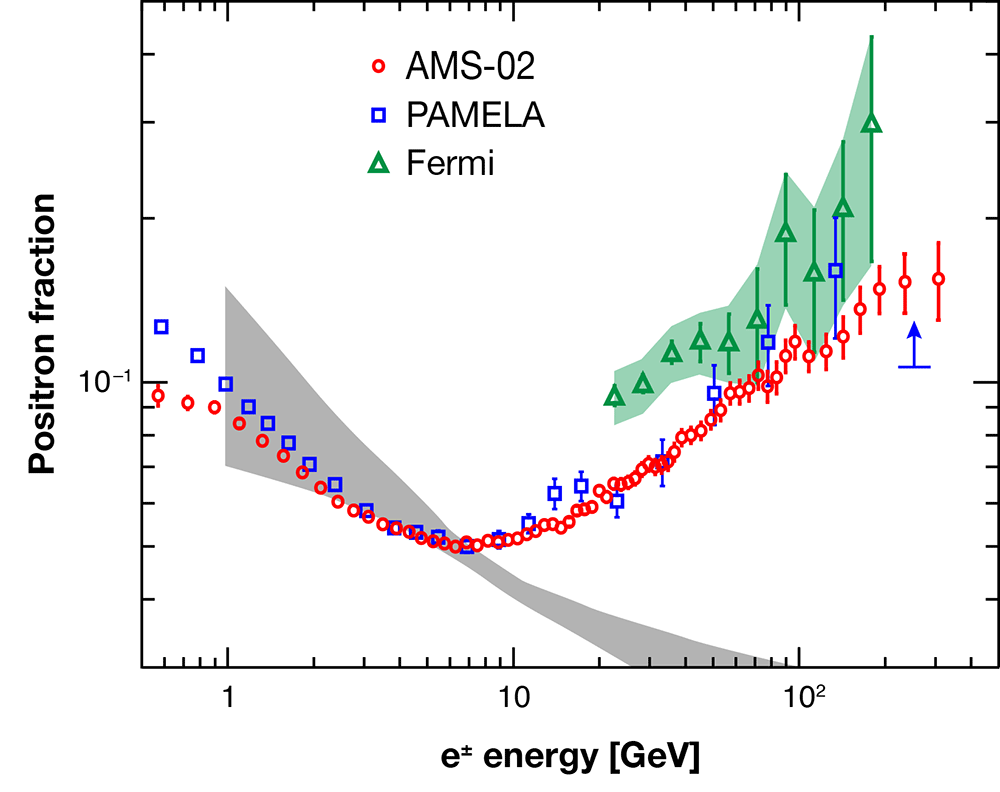
\includegraphics[width=0.5\textwidth]{figs/motivation/pamela.png}
    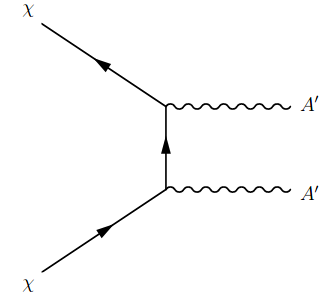
\includegraphics[width=0.35\textwidth]{figs/motivation/dm_annihilation.png}
    \caption{Left: The results from PAMELA, AMS, and Fermi-LAT showing the positron fraction excess (above the expected calculation from cosmic rays in grey) at above $\sim 10$ GeV \cite{Coutu:2013}. Right: The Feynman diagram for the dark matter annihilation into two $\aprime$s which subsequently decay into $\epem$ pairs. This provides an explanation for positron fraction excess. This explanation has since been disfavored. Note that S-channel annihilations are possible but not considered since they are suppressed by a factor of $\epsilon$; however, the cross-section for annihilations into two $\aprime$s is determined by $\alpha_{D}$ (the coupling of the $\aprime$ to dark matter particles) which can be arbitrarily large. 
    }
    \label{fig:pamela}
\end{figure}

There are two specific historical anomalies that generated much interest in the heavy photon hypothesis among the communities of particle physicists and astrophysicists. In 2008, the Payload for Antimatter Matter Exploration and Light-nuclei Astrophysics (PAMELA) measured an anomalous excess of positron fraction $\phi (e^+)/(\phi (e^+) +\phi (e^-) )$ above $\sim 10$ GeV that was inconsistent with the expectation from secondary production from cosmic-ray nuclei interactions with interstellar gas \cite{Adriani:2008zr} \cite{ackermann2012}. Further measurements from the Fermi Large Area Telescope and the Alpha Magnetic Spectrometer (AMS) not only confirmed this anomaly, but extended it to even higher energies of $\sim 200$ GeV \cite{aguilar2013}. These measurements are shown in Fig. \ref{fig:pamela}. 

The implied annihilation cross-section from the observed positron fraction excess is larger than one would expect from a dark matter thermal relic ($\langle \sigma v \rangle \sim 3 \times 10^{-26}\mathrm{cm}^3 \mathrm{s}^{-1}$). However, the scenario in which dark matter annihilation occurs through a heavy photon mediator shown in Fig. \ref{fig:pamela} is particularly appealing since a so-called ``Sommerfeld enhancement'' can occur in which the cross-section is dependent on the inverse of velocity ($\langle \sigma v \rangle \sim 1/v$) \cite{ArkaniHamed:2008qn}. Thus low-velocity interactions (e.g. dark matter collisions in the galactic halo) are enhanced while still preserving the dark matter freeze-out scenario (described in Sec. \ref{sec:ldm}) with the observed dark matter relic abundance. In addition, antiproton cosmic ray yield does not increase with energy which motivates heavy photons with $m_{\aprime} < 2m_p$ where decays to proton-antiproton pairs are kinematically forbidden. Thus, the MeV-GeV heavy photon mass range is highly motivated by both the Sommerfeld enhancement and observations of annihilation into hadrons.

This anomaly is now disfavored for several reasons. A larger AMS dataset shows a softer positron spectrum that is more consistent with a pulsar origin for cosmic ray positron excess than a heavy photon interpretation; however, this does not exclude the possibility of heavy photons decaying into intermediate states before an $\epem$ final state \cite{Cholis:2013psa}. In addition, measurements by the Planck satellite put strong constraints on the dark matter annihilation rate at recombination, thus making the heavy photon explanation of the PAMELA anomaly unlikely \cite{Ade:2015xua}.

In addition to the positron cosmic ray excess, heavy photons were originally motivated by the measurement of the magnetic momentum of muons ($a_{\mu}=(g-2)/2$, or simply known as $g-2$) which deviates by more than 3 standard deviations away from the predicted value from the SM. This can be explained by a contribution of the heavy photon to the muon magnetic moment for a heavy photon within a certain range of parameter space shown in green in Fig. \ref{fig:projections}. In addition, the excellent agreement between the corresponding magnetic moment of the electron and the SM excludes the region in red. This favored region for a heavy photon explanation of the anomalous magnetic moment of the muon has since been ruled out by several experiments both for visible and invisible decays.

A heavy photon hypothesis for these two anomalies has since been ruled out. Even though some of the original motivations for dark sector searches such as the anomalous positron excess from PAMELA and the muon G-2 anomaly are no longer favored, motivations for searching for such a particle remain particularly in models involving light dark matter.

%muon G-2 \cite{Gaiser:1982yw}

%Anomalous Muon Magnetic Moment\cite{Bennett:2006fi}

%Fermi \cite{Hooper:2010mq}

%Fermi LAT \cite{Abazajian:2010zy}

%Fermi \cite{Goodenough:2009gk}

%Pulsar \cite{yin2013}

%Pulsar \cite{linden2013}

%Planck \cite{Adam:2015rua}

\clearpage

\section{Light Dark Matter}\label{sec:ldm}

\begin{figure}
    \centering
    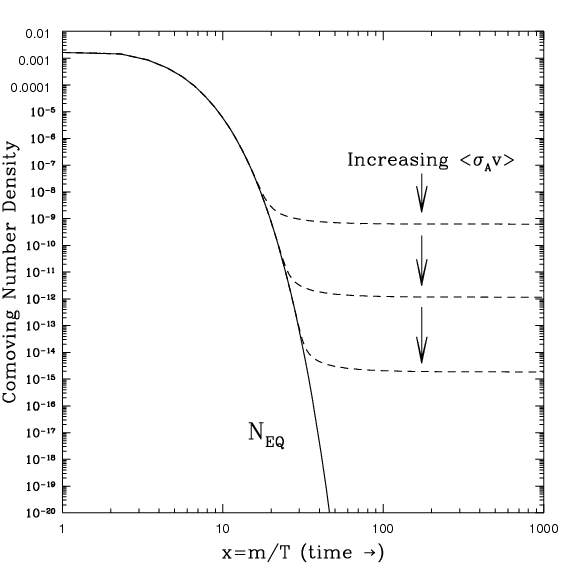
\includegraphics[width=0.85\textwidth]{figs/motivation/thermalfreezeout.png}
    \caption{The mechanism of thermal freeze-out in which dark matter and SM matter are in thermal equilibrium in the early universe. As the universe cools ($x$-axis), the relic abundance of dark matter ($y$-axis) is depleted by self-annihilation until enough cooling occurs and the dark matter relic abundance is set \cite{Jungman_1996}.}
    \label{fig:freezeout}
\end{figure}

Heavy photons are connected to a variety of models of light dark matter, that is dark matter on the MeV-GeV scale (or sub-GeV scale) where stable massive SM particles are known to exist, as well as self-interacting dark matter. In order to understand the potential connection between light dark matter and heavy photons, one must first understand the mechanisms of thermal dark matter and its connection to the amount of dark matter relic abundance. This connection is referred to as ``thermal freeze-out'' (which was alluded to in Chp. \ref{chap:intro}) and the simplest annihilation of thermal freeze-out as shown in Fig. \ref{fig:freezeout} goes as follows.

%The galactic rotation curves and the CMB evidence shows that the same dark matter that is around today was the same dark matter around in the early universe. In addition, they are about the same... gives compelling motivation for a thermal origin of dark matter, that is it was in thermal equilibrium in the early universe with Standard Model particles. One method of thermal dark matter, called thermal freeze-out, is annihilation... This mechanism is illustrated in Fig. \ref{fig:freezeout}.

%Additional fundamental forces gives rise to...

\begin{enumerate}
  \item The whole universe began in a hot dense state with some amount of SM matter ($\Omega_{SM}$) and some density of dark matter ($\Omega_{DM}$) colliding in thermal equilibrium.
  \item Through an unspecified mechanism, dark matter particles annihilate with one another into SM particles and through the same mechanism SM also annihilate into dark matter particles. This occurs in thermal equilibrium. For simplicity, dark matter self-interactions are assumed to have an no effect on this mechanism.
  \item Throughout this process, the universe expands and cools which decreases the rate of dark matter-SM interactions. Eventually, the universe cools enough to stop the SM annihilation into dark matter particles; however, the dark matter annihilation into SM particles persists. Thus, over this short time the amount of dark matter is continually depleted.
  \item As the universe continues to expand, eventually these dark matter annihilations stop as dark matter completely decouples from the SM. At this point, the amount of dark matter called the ``relic abundance'' is set at a fixed value. Measurements from a variety of astrophysical sources described in Sec. \ref{sec:observations} put the relative relic abundance $\Omega_{DM}=$85\% of the total matter in the universe. In addition, there is an inverse relationship between the annihilation cross-section and the relic abundance ($ \langle \sigma v \rangle \propto \frac{1}{\Omega_{DM}}$) such that the larger the dark matter annihilation cross-section the more it will be depleted.
\end{enumerate}

From the observed relic abundance (measurements from the CMB and Type 1a Supernovae), using the inverse relationship the expected annihilation cross-section can be computed as $\langle \sigma v \rangle \sim 3 \times 10^{-26}\mathrm{cm}^3 \mathrm{s}^{-1}$. In addition, the annihilation cross-section can be related to the dark matter particle mass and the mass of mediator (such as the $Z$ boson in this case) as follows:

\begin{equation}
    \langle \sigma v \rangle \propto \frac{m_{DM}^2}{m_Z^4}
    \label{eqn:dmcs}
\end{equation}

One can solve for the dark matter particle mass and see that such a mechanism gives a mass in the 100 GeV range. This mass scale and cross-section is typical of what one would expect from weak sector particles such as $W$ bosons, $Z$ bosons, or Higgs bosons providing a hint that a dark matter particle could be a particle that interacts weakly with SM particles. These dark matter candidates are named ``Weakly Interacting Massive Particles'' (WIMPs), and this mass and cross-section computation is such a remarkable coincidence that this is famously referred to as the ``WIMP Miracle.'' However, a major difference between WIMPs and weak-scale SM particles is that WIMPs must be stable in order to be a dark matter candidate whereas weak-scale SM particles are unstable. In addition, in order to resolve the hierarchy problem, models of Supersymmetry (SUSY) were developed, and many of these models described WIMP-like objects.

Because of this, over the past few decades much of the focus of the particle physics and astrophysics communities has been on both direct detection experiments and colliders such as the Large Hadron Collider (LHC) searching for WIMP-like dark matter and SUSY on the $\sim$100 GeV-scale. However, to date of publication, neither WIMPs nor SUSY have been discovered and accessible parameter space for these models is shrinking. Specifically, direct detection experiments are approaching the so-called neutrino floor where the direct detection of neutrinos with the detector medium become indistinguishable from dark matter recoils, thus searches of this type will no longer be possible. In addition, the LHC will probe the most favorable models of SUSY within the next few years.

As a way to complement the SUSY-WIMP dark matter searches, it is reasonable to search for dark matter at the mass scale where known stable SM particles, such as electrons and protons, exist. If one naively computes the relic abundance of potential dark matter particles on the MeV - GeV scale with an electroweak mediator using Eq. \ref{eqn:dmcs}, the calculation results in an annihilation cross-section far smaller than is expected from the simplest mechanisms of thermal equilibrium. And because the annihilation cross-section is proportional to the inverse of the relic abundance, this mass scale crosses the threshold of the so-called Lee-Weinberg bound at $\sim$2 GeV such that dark matter candidates below this bound will result in an overproduction of dark matter.\footnote{When computing any mechanism of thermal origins of dark matter, and overproduction above the observed relic abundance is never allowed. However, an underproduction of dark matter is allowed since another mechanism can compensate the remaining dark matter relic abundance.} Of course, this computation assumes only interactions mediated through SM bosons such as $W$ bosons, $Z$ bosons, and Higgs bosons.

As a way to circumvent the Lee-Weinberg bound, one could postulate an annihilation mechanism through a new, comparably light mediator. This would provide another degree of freedom in Eq. \ref{eqn:dmcs} and allow for this simple mechanism to produce the observed dark matter relic abundance. Thus, any thermal dark matter model on the MeV-GeV scale, called ``light dark matter'', requires an additional boson beyond the SM. A heavy photon is a simple and natural candidate that could mediate dark matter annihilations in the early universe (though collisions in the galactic halo occur at an enhanced rate because of the Sommerfeld enhancement). Beyond this simple mechanism, heavy photons are connected with more complicated models of dark matter that allow for more complex structure and interactions within the so-called ``dark sector'' - the sector of all particles responsible for the 85\% of dark matter. Due to the kinetic mixing between the heavy photon and the SM photon, heavy photons would provide an indirect mechanism (called a ``vector portal'') to probe the particles and interactions in this dark sector.

In addition to mechanisms of thermal dark matter and a vector portal, heavy photons are motivated by a variety of self-interacting dark matter models where dark sector particles are allowed to interact with other dark sector particles.\footnote{These dark matter self-interaction can be mediated by heavy photons or by other additional mediators in the dark sector. In contrast, the minimal WIMP model does not allow for additional self-interactions.} Excesses in both gamma ray and X-ray spectra can provide hints of dark matter self-interactions potentially mediated by heavy photons. The Fermi-LAT telescope has observed an extended emission in the gamma ray spectrum originating from the galactic center. There are several models that explain this including pulsars, energetic protons accelerated by a super-massive black hole, and dark matter annihilations into SM particles. The dark matter annihilation can be explained through a heavy photon model, much like what was explained for the original observed positron fraction anomaly by PAMELA. An excess in the X-ray spectra at 3.5 keV from several galaxy clusters has been explained in a model called ``eXciting Dark Matter'' (XDM). In this model, self-interacting dark matter can collide via a heavy photon and excite dark matter ($\chi^* \chi^*$) and its subsequent de-excitation emits an observable 3.5 keV X-ray ($\chi^* \rightarrow \chi \gamma$).

Along the same lines of self-interacting dark matter, collisionless dark matter has historically failed to account for detailed simulations of dark matter of galactic halos. Often these problems can be resolved by self-interacting dark matter with a velocity-dependent cross-section which is consistent with a heavy photon hypothesis which would otherwise be constrained by high-velocity collisions such as the Bullet Cluster shown in Fig. \ref{fig:dm} \cite{Markevitch_2004}.

For instance, there are observations in which Milky Way dwarf satellite galaxies have smaller rotational velocities than predicted by these simulations for dark matter subhalos. This is called the ``too big to fail'' problem and it suggests that the rotational velocities are actually smaller than predicted, these massive subhalos fail to create these dwarf galaxies, or these massive subhalos simply do not exist. Self-interacting dark matter provides a solution via the first possibility as it can naturally reduce the central densities of subhalos (and hence reducing their rotational velocities). In addition, collisionless dark matter dark matter fails to resolve the so-called ``cusp-core problem'' in which the observed matter density profiles of galaxies are better modeled with a constant density core from self-interacting dark matter than models from collisionless dark matter. Heavy photons in the mass range 1 - 10 MeV over a wide range of $\epsilon^2$ are motivated by self-interacting dark matter. There are, however, other explanations of these phenomena that do not involve self-interacting dark matter such as baryonic outflows in galaxies that may also produce similar cored distributions by transferring energy to dark matter. As these simulations develop and improve over time, these conflicts of collisionless dark matter may be resolved.

%Another cosmological motivation for heavy photons involves the cosmic dawn. 
The Experiment to Detect the Global EoR Signature (EDGES) observed a strong absorption profile of 21 cm hydrogen  \cite{FRASER2018159}. This indicates that hydrogen gas is colder than expected from standard cosmological conditions. One possible explanation is dark matter on the $\sim 10$ MeV scale scattering with SM matter through an $\aprime$ mediator during the first stellar formation (the cosmic dawn).

Finally, heavy photons are motivated as an explanation of an anomaly from nuclear physics in which a significant excess was observed in the angular spectrum for the internal pair creation for an excited state to ground state transition of Be8 nuclei \cite{Krasznahorkay_2016}. This was interpreted as a new protophobic (a different coupling to different quark flavors) boson called ``X17''  \cite{Feng_2017}. A similar anomaly was found by the same group for He3 nuclei which could be explained by the same hypothetical boson \cite{krasznahorkay2019new}. However, recent results from NA64 at CERN have excluded some portion of the expected parameter space, but have not completely ruled it out yet \cite{Banerjee_2019}. %\textcolor{red}{More detail about He3. Lepto-phobic?}



%Light DM \cite{Hooper:2012cw}

%X-ray spectrum \cite{Bulbul:2014sua}

%exciting DM \cite{Finkbeiner:2014sja}

%Gamma rays from galactic center \cite{hooper2011}

%DM and syncrotron radiation \cite{linden2011}

%DM from galactic center \cite{abazajian2012}

%Fermi Bubbles \cite{hooper2013}

\clearpage

\section{Signatures of A's}\label{sec:signatures}

 \begin{figure}
    \centering
    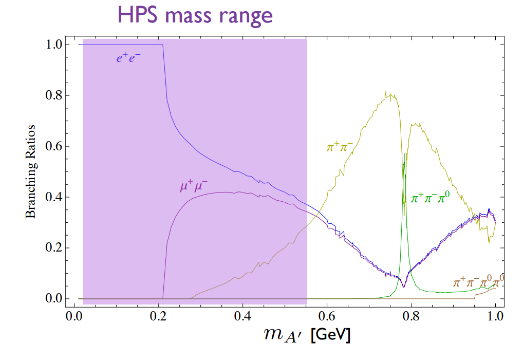
\includegraphics[width=0.85\textwidth]{figs/motivation/br.png}
    \caption{The branching ratio for heavy photon decays to SM particles as a function of mass. This assumes no decays into dark sector particles.}
    \label{fig:br}
\end{figure}

According to the minimal heavy photon model, kinetic mixing is the only coupling to the SM. One can also assume decays to dark sector particles are forbidden (i.e. $2m_d>m_{\aprime}$), thus the focus will be on visible decays (i.e. SM particles).\footnote{If one relaxes this assumption, the possible decay scenarios become more complicated. Decays to invisible particles become possible and searches for missing mass or missing momentum must be performed.} Under this assumption, the branching ratio of heavy photon decays to visibles as a function of mass in the MeV-GeV range is shown in Fig. \ref{fig:br} which is derived by the ratio of cross-sections as a function of center-of-mass energy for different final states of $\epem$ interactions.

The heavy photon decay width is given by:

\begin{equation}
    \Gamma=\frac{N_{eff}m_{\aprime}\alpha \epsilon^2}{3}
    \label{eqn:Gamma}
\end{equation}

where $N_{eff}=2+R(m_{\aprime})$ and the function $R(Q)$ is given by

\begin{equation}
    R(Q)=\frac{\sigma(e^+e^- \rightarrow \mathrm{hadrons},Q)}{\sigma(e^+e^- \rightarrow \mu^+ \mu^-,Q)}
    \label{eqn:r}
\end{equation}

For $m_{\aprime}<2m_{\mu}$, $N_{eff}=1$ since the only kinematically allowed SM decay is to $\epem$ pairs.\footnote{This is true for most of the parameter space covered by HPS, though the mass range at higher beam energies for HPS does cross the dimuon threshold.} Since the fractional decay width $\Gamma/m_{\aprime}$ is proportional to $\alpha \epsilon^2$, the small $\epsilon^2$ will result in a very narrow decay width, and the heavy photon will appear as a sharp resonance.

The corresponding product of livetime and the speed of light (the $c\tau$ value) is related to the inverse of the decay width in Eq. \ref{eqn:Gamma} by:

%\begin{equation}
%    \tau=\frac{\hbar}{\Gamma}=\frac{3\hbar}{N_{eff}m_{\aprime}\alpha \epsilon^2}
%    \label{eqn:tau}
%\end{equation}

\begin{equation}
    c\tau=\frac{\hbar c}{\Gamma}=\frac{3\hbar c}{N_{eff}m_{\aprime}\alpha \epsilon^2}
    \label{eqn:ctau}
\end{equation}

The decay length in the laboratory frame is related to $c\tau$ value by a factor of relativistic $\gamma$ but is not universal as it will depend on the type of experiment (e.g. fixed target experiment vs. a collider experiment). But, for sufficiently small $\epsilon$, the decay length becomes measureable for both types of experiments with excellent vertex resolution (typically fixed target experiments, but sometimes colliders as well) and beam dump experiments.

Finally, the rate of heavy photon production is directly proportional to the corresponding process for virtual photons at a given heavy photon mass. Thus, there exist an irreducible background with identical kinematics for a given heavy photon production. The only directly distinguishable feature is the fact that the heavy photon is on-shell and can have a finite, and hence measureable, livetime. The ratio of the $\aprime$ differential cross-section for a given $m_{\aprime}$ and $\epsilon$ to the cross-section of the corresponding virtual photon process integrated over the narrow mass range $m_{\aprime} \pm \frac{\delta m}{2}$ is given by \cite{Bjorken:2009mm}:

\begin{equation}
    \frac{\mathrm{d}\sigma(X \rightarrow \aprime Y \rightarrow ZY)}{\mathrm{d}\sigma(X \rightarrow \gamma^* Y \rightarrow ZY)} = \left( \frac{3\pi \epsilon^2}{2 N_{eff}\alpha} \right) \left( \frac{m_{\aprime}}{\delta m} \right)
    \label{eqn:radiatives}
\end{equation}

The specific virtual photon process related to HPS is discussed in more detail Sec. \ref{sec:backgrounds}. If an experiment can directly measure the rate of the corresponding virtual photon process, the expected rate of heavy photon production can be normalized in a data-driven way. 

\clearpage

\section{Overview of Searches}\label{sec:searches}

 \begin{figure}
    \centering
    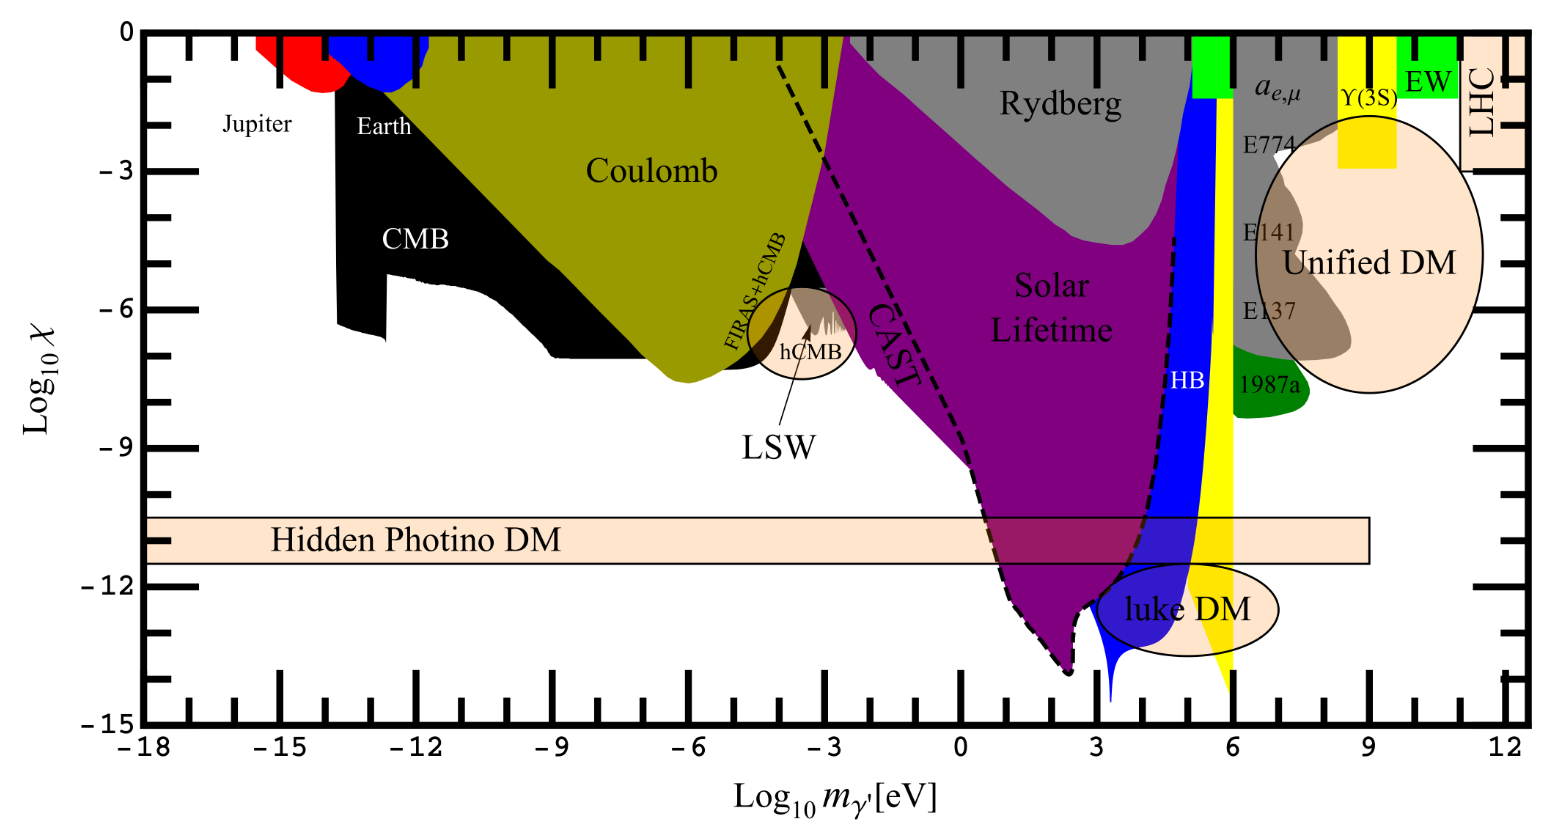
\includegraphics[width=0.95\textwidth]{figs/motivation/constraints.png}
    \caption{Existing constraints of heavy photons on the whole parameter space \cite{Jaeckel_2010}. The constraints come from a variety of sources including astrophysical measurements, precision QED, and particle accelerator-based experiments. The regional labeled ``unified DM'' is of particular interest to dark matter for reasons described in Sec. \ref{sec:ldm} and Sec. \ref{sec:history} and will be the focus. Note that the notation in this plot is such that $\epsilon \rightarrow \chi$ and $\aprime$ is denoted as $\gamma'$.}
    \label{fig:constraints}
\end{figure}

The parameter space for heavy photons is large, and current heavy photon constraints from various astrophysics measurement, precision QED, and accelerator-based experiments are summarized in Fig. \ref{fig:constraints} \cite{Jaeckel_2010}. There is a much narrower region of partially unexplored parameter-spaced that is theoretically favorable with sub-GeV dark matter models. This parameter space is typically probed by accelerator-based experiments in which a beam of high energy particles (e.g. electron, protons, etc.) are collided with material or another beam in order to produce heavy photons.

The common production methods are through dark bremsstrahlung ($e^-Z \rightarrow e^- Z \aprime$), Drell-Yan ($q\bar{q} \rightarrow \gamma \aprime$), $\epem$ annihilation ($\epem \rightarrow \gamma \aprime$), and meson decays (such as $\pi^0 \rightarrow \gamma \aprime$ $\eta \rightarrow \gamma \aprime$ $\phi \rightarrow \eta \aprime$). Once heavy photons are produced, experiments are designed and built to detect heavy photons often by measuring their decay products. Common detection signatures include a mass resonance of the SM decay products, missing mass or momentum (heavy photons decay to dark sector particles and cannot be detected directly), and displaced vertices from long-lived heavy photons. 

Different types of experiments and facilities are designed to utilize these production and detection methods. These include complementary searches from colliders, thin fixed targets, and beam dumps from facilities that utilize protons beams, ion beams, electron beams, and positron beams. In general, fixed targets and beam dump experiments are higher luminosity and able to probe smaller $\epsilon$ while colliders with a high center-of-mass energy can probe larger masses.

\subsection{Colliders}\label{sec:colliders}

Searches for heavy photons at colliders mostly come from flavor factories that produce heavy photons through meson decays, but also through $\epem$ annihilation, Drell-Yan, and even displaced vertices.

Among the experiments that utilize high-luminosity $\epem$ colliders to search for heavy photons are BaBar, KLOE and KLOE-II, and Belle-II. Each of these experiments were run at different center-of-mass energies and thus searched at complementary masses. BaBar was run at the PEP-II B-Factory at SLAC and heavy photon searches were performed using upsilon decays ($\Upsilon \rightarrow \gamma \aprime$) and then heavy photon decays into $\mu^+ \mu^-$ final states \cite{Aubert:2009cp}. In addition to visible final states, BaBar has searched for heavy photon decays into invisibles \cite{PhysRevLett.119.131804}. In the future, Belle-II will also be able to search for invisible decays and is projected to improve upon the results from BaBar \cite{pietro2018data}. KLOE and KLOE-II were run at the DA$\Phi$NE$\phi$ factory and search for $\phi$ meson decays ($\phi \rightarrow \eta \aprime$) and then heavy photon decays into $\epem$ and $\mu^+ \mu^-$ final states as well as dipion decays \cite{Babusci:2012cr} \cite{Archilli:2011zc} \cite{Mandaglio:2017kiv}.

Proton colliders such as the Large Hadron Collider (LHC) at CERN which houses experiments such as ATLAS  \cite{Aad:2012tfa}, CMS \cite{Chatrchyan:2012xdj}, and LHCb can search for meson decays and forms of ``dark showering''. Since these experiments are run at a higher center-of-mass energy than any other current experiment, these experiments can probe the largest $\aprime$ mass space. 

Specifically, for heavy photon masses below the dimuon threshold LHCb can search for heavy photons in the $D^* \rightarrow D^0 \aprime$ channel decays into $\epem$ final states \cite{Ilten:2015hya} \cite{Ilten:2016tkc} \cite{PhysRevLett.120.061801}. For heavy photon masses above the dimuon threshold, LHCb can search for heavy photon decays into a $\mu^+ \mu^-$ final state. In addition, LHCb can perform a displaced vertex search for $\eta$ decays in a heavy photon and ($\eta \rightarrow \gamma \aprime$) then for a long-lived heavy photon that decays into a $\mu^+ \mu^-$ final state. Future upgrades to LHCb, specifically a trigger-less readout that allows for online reconstruction, will enable a search for displaced vertices with an $\epem$ final state with projected sensitivity competitive with the HPS displaced vertex search.

Lower energy proton colliders such as WASA at COSY searched for neutral pion decays into heavy photons ($\pi_0 \rightarrow \gamma \aprime$) and heavy photon decays into $\epem$ final states. PHENIX at the Relativistic Heavy Ion Collider (RHIC) at Brookehaven uses both proton-proton and deuterium-gold nuclei ($d+$Au) collisions to produce neutral mesons that decay into heavy photons ($\pi_0 \rightarrow \gamma \aprime$ and $\eta \rightarrow \gamma \aprime$) which then decay into $\epem$ final states \cite{Adare:2014mgk}. 

%Mu3e \cite{Echenard:2014lma}

%e-p colliders \cite{Freytsis:2009bh}
\subsection{Beam Dumps}\label{sec:beamdump}

 \begin{figure}
    \centering
    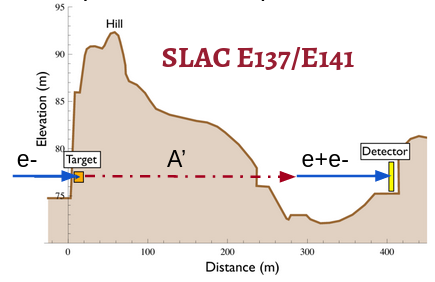
\includegraphics[width=0.55\textwidth]{figs/motivation/beamdump.png}
    \caption{A schematic of beam dump experiments SLAC E137 and E141 which searched for long-lived particles that decay in a region several hundred meters from the target.}
    \label{fig:beamdump}
\end{figure}

As previously stated, heavy photons with sufficiently small couplings will be long-lived. This property can be exploited by beam dump experiments where a high intensity electron or proton beam is ``dumped'' onto a thick target, and a search for heavy photon decays to visible particles can be performed. If the beam dump is sufficiently thick enough, this will filter all SM background and any decay within a specific volume would be clear evidence for a new long-lived particle. Otherwise, the decay products must be reconstructed to measure their decay position to distinguish SM processes from potential new processes.

Several general-purpose electron beam dump experiments that were originally designed and run to search for axion-like and Higgs-like particles such as E137 and E141 at SLAC \cite{Bjorken:1988as}, E774 at Fermilab \cite{bross1991}, KEK in Japan \cite{konaka1986}, and an experiment at Orsay reinterpreted previously taken data to show constraints for heavy photons \cite{andreas2012}. NA64 is a recent electron beam dump at CERN \cite{Banerjee_2019}. These experiments produce heavy photons by dark bremmstrahlung, a process related to ordinary photon bremmstrahlung. Future electron beam bumps include the Beam Dump eXperiment (BDX) \cite{battaglieri2016dark}.

Similar constraints can be set from a proton beam dump experiment where heavy photons are produced by either the decay of neutral mesons produced at the target or proton bremsstrahlung such as the U70 accelerator. Future proton beam dump experiments include a SHiP at CERN \cite{Alekhin:2015byh} which is a general-purpose dark sector experiment, SeaQuest at Fermilab (soon to be SpinQuest or DarkQuest) which is is typically used for nuclear physics experiments \cite{Gardner:2015wea}, and COHERENT at Oak Ridge \cite{PhysRevD.92.095005}. Finally, several short-baseline neutrino experiments at Fermilab that utilize proton beam dumps such as MiniBooNe can search for heavy photons \cite{Aguilar_Arevalo_2017} \cite{acciarri2015proposal}.

%Proton beam dump \cite{Blumlein:1990ay}

%Proton beam dump \cite{Blumlein:1991xh}

%Beam dumps \cite{Blumlein:2011mv}

%Beam dumps \cite{Blumlein:2013cua}

\subsection{Thin Fixed Target}\label{sec:fixedtarget}

Fixed target experiments are much like beam dump experiments; however unlike beam dump experiments, fixed target experiments are designed with a much thinner target to detect the decay products of relatively short-lived $\aprime$s. As a result, fixed target experiments must have the ability to reconstruct vertices to distinguish the relatively short-lived $\aprime$s from SM particles. %which has the advantage of enabling both prompt and long-lived searches for heavy photons. %which allows for most SM particles to interact with the detector that would otherwise be filtered by a beam dump. As a result, fixed target experiments must have the ability to reconstruct these SM particles which has the advantage of enabling both prompt and long-lived searches for heavy photons.

Fixed target experiments utilize an electron beam to produce $\aprime$s using the same dark bremmstrahlung mechanism as beam dump experiments. A Prime EXperiment (APEX) is a fixed target experiment at Jefferson Laboratory that uses an electron beam to detect the $e^+e^-$ decay products from an electro-produced heavy photon \cite{Essig:2010xa} \cite{Abrahamyan:2011gv}. It uses a septum magnet to separate $e^+e^-$ pairs into two calorimeters (HRS spectrometer in Hall A) whose measurements are used to compute the invariant mass. In addition, the A1 spectrometer at the Mainz Microtron also searches for heavy photon decays to $\epem$ pairs \cite{Merkel:2014avp}. Several additional electron beam fixed target experiments are planned including DarkLight using the Low-Energy Recirculator Facility at JLab and MAGIX at the Mainz Energy-Recovering Superconducting Accelerator.

Future experiments such as the Light Dark Matter eXperiment (LDMX) at SLAC search for heavy photons through a production of dark bremmstrahlung and a subsequent decay into invisibles \cite{kesson2018light}. The search is for a missing momentum signature by precision measurements of the recoil electron momentum. Rare photo-nuclear processes that can mimic a missing momentum and a missing energy signature are vetoed by a large hadronic calorimeter. The design of the LDMX apparatus is shown in Fig. \ref{fig:ldmx}.

 \begin{figure}[!h]
    \centering
    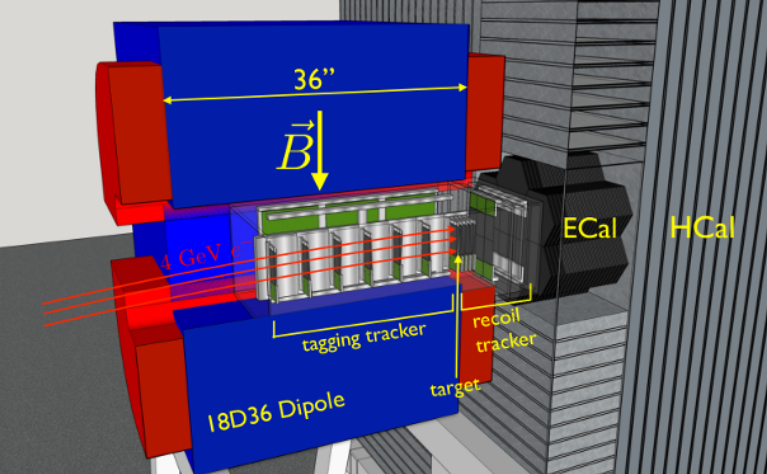
\includegraphics[width=0.5\textwidth]{figs/motivation/ldmx.png}
    \caption{The Light Dark Matter eXperiment (LDMX) searches for heavy photon decays to invisibles by measuring the recoil electron momentum and searching for missing momentum. The apparatus includes a tagging tracker, recoil tracker, an Ecal, and an Hcal.}
    \label{fig:ldmx}
\end{figure}

In addition to electron beams, positron beams are also used in fixed target experiments to search for heavy photons through $\epem$ annihilation. These searches utilize monophoton final states ($\gamma \aprime \rightarrow \gamma \chi \chi^*$) such that a missing mass search can be performed. Proposed experiments of this type include PADME at INFN Frascati and VEPP-3 at the Budker Institute at Novosibirsk \cite{Wojtsekhowski:2012zq}. The proposed Missing Mass A-Prime Search (MMAPS) at Cornell is a similar style missing mass search with a $\epem \rightarros \gamma \aprime$ \cite{Alexander2016}.

Proton fixed target experiments such as NA48/2 at the Super Proton Synchrotron (SPS) at CERN search for meson decays into heavy photons (specifically $K^{\pm} \rightarrow \pi^{\pm} \pi^0$; $\pi^0 \rightarrow \aprime$), that then decay to $e^+e^-$ pairs by utilizing a beryllium target to produce a Kaon beam ($K^{\pm}$) \cite{Batley:2015lha}. In addition, the HADES measures potential heavy photons from meson decays (specifically $\pi_0 \rightarrow \gamma \aprime$, $\eta \rightarrow \gamma \aprime$, $\Delta \rightarrow N \aprime$) and $\epem$ final states by using a a variety of both hydrogen and niobium (Nb) targets \cite{Agakishiev:2013fwl}.

Finally, the Heavy Photon Search (HPS) utilizes an electron beam to produce $\aprime$s through dark bremstrahlung and searches for $\epem$ daughter particles from $\aprime$ decays. HPS is unique in that it reconstructs both the mass and vertex positions with excellent precision which enables searches for both prompt decays and secondary vertices from heavy photons with a short decay length in the range of 1-10 cm in the laboratory frame. The heavy photon theoretically favored parameter space assuming visible decays as well as the existing constraints from the experiments described above and future projections from HPS (shown with green contours) is shown in Fig. \ref{fig:parameterspace}. The red band in the figure is a region favored by a variety of dark matter models that consist of an $\aprime$ mediator. The region is composed of several lines, and each line corresponds to a thermal target of a specific dark matter model in which that particular type of dark matter with those $\aprime$ parameters compromises 100\% of the dark matter ($\aprime$s existing above the line results in an underproduction of dark matter and below results in an overproduction). These thermal targets are a strong motivation for the displaced vertex search for HPS; HPS is currently the only experiment that can probe this territory.

%\textcolor{red}{Also, TREK at J-PARC \cite{Albrow:2016ibs} (using a stopped kaon beam)} 

\begin{figure}
    \centering
    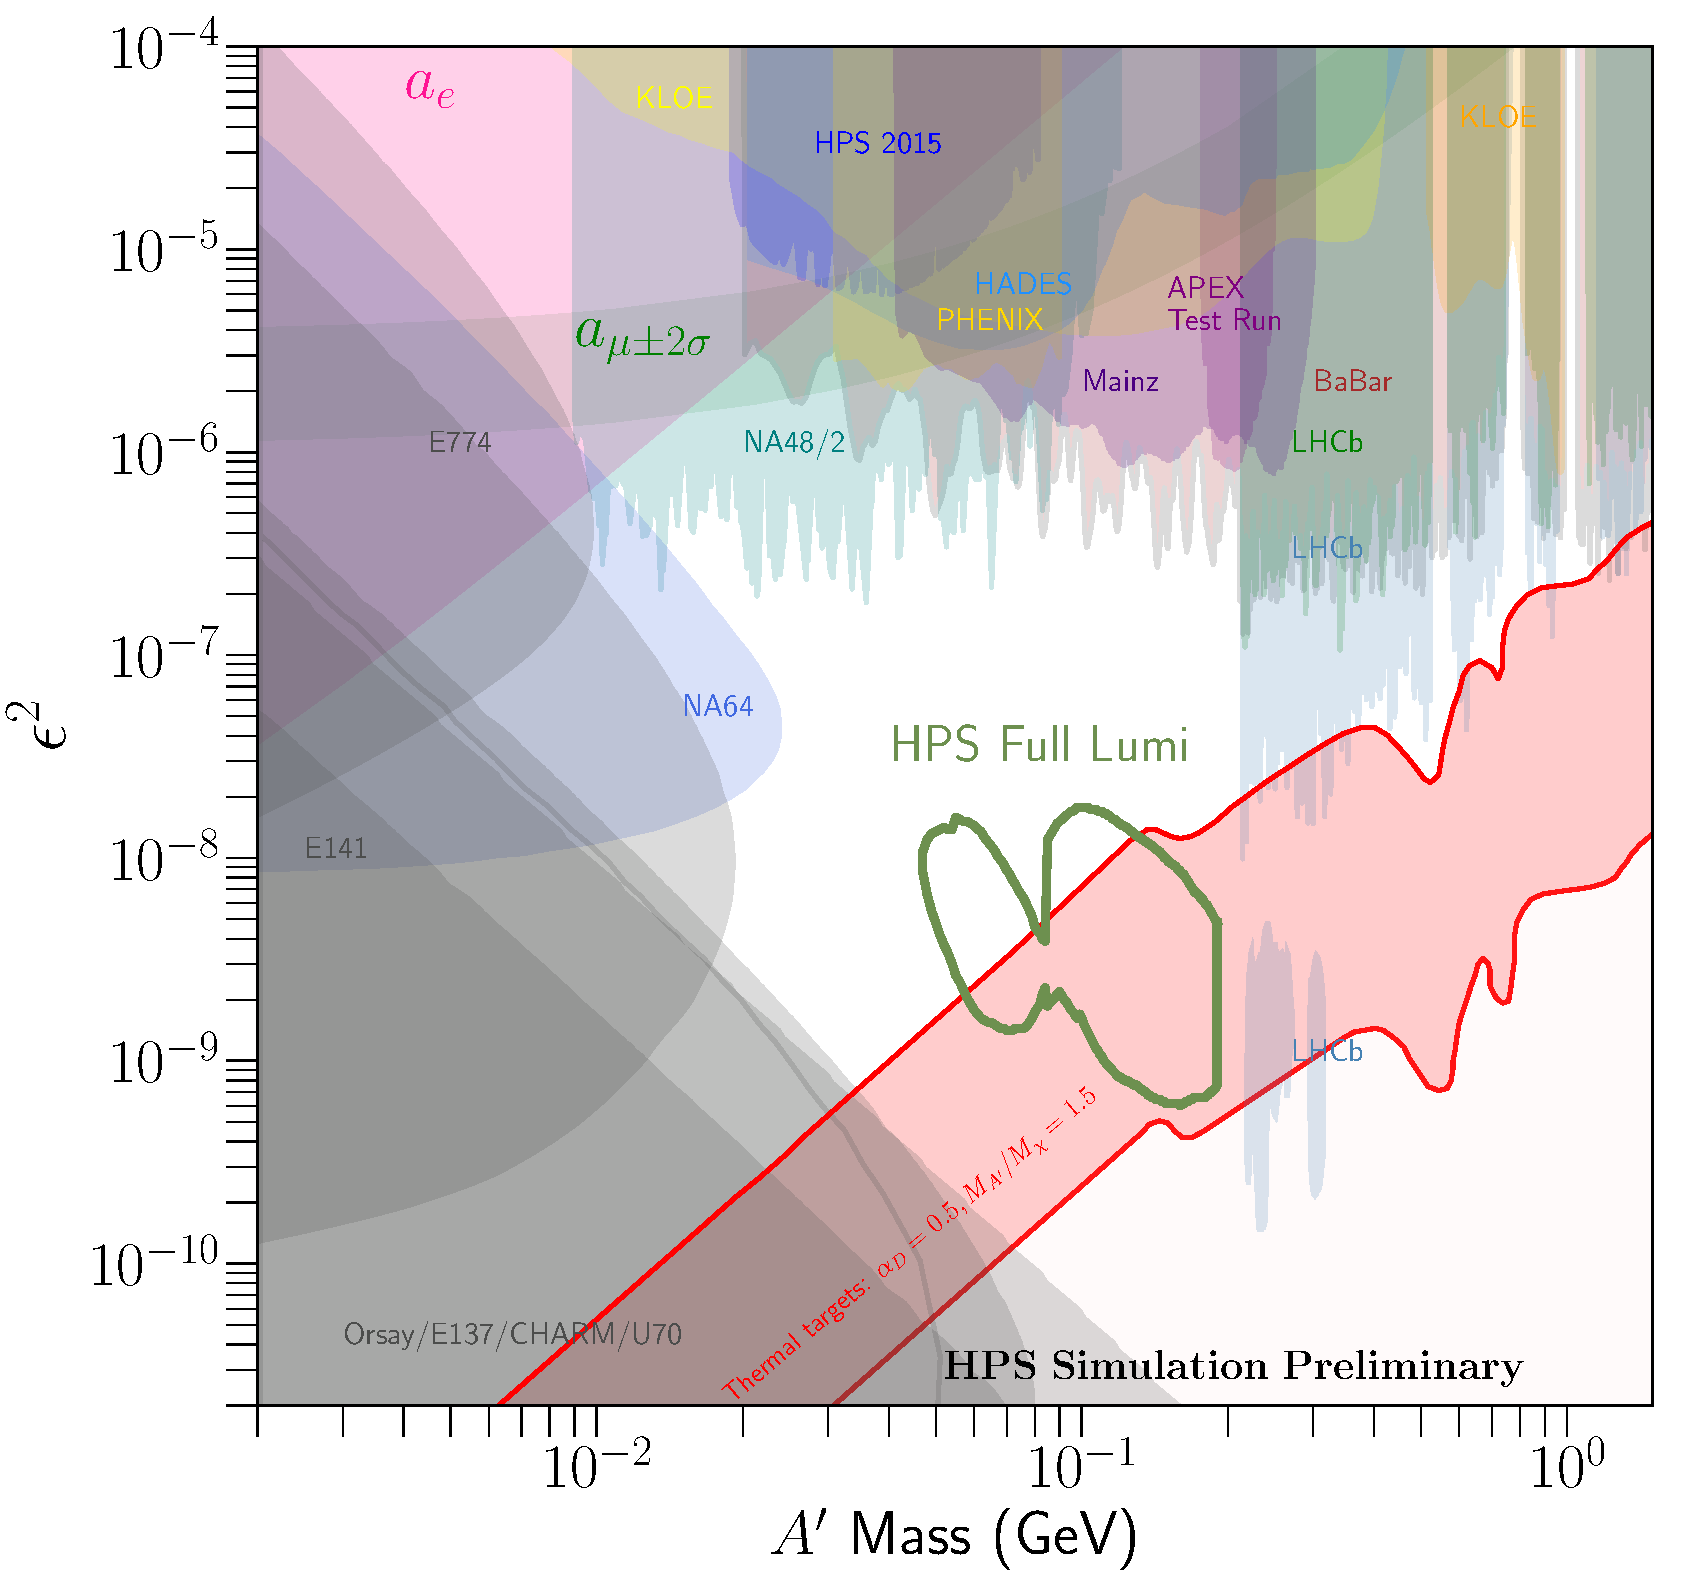
\includegraphics[width=0.85\textwidth]{figs/upgrades/reach_full_lumi.pdf}
    \caption{Existing constraints for heavy photons from experiments described in Sec. \ref{sec:searches}. These exclusions assume the mass hierarchy $m_{\aprime}<2m_{DM}$, and searches assuming the inverse mass hierarchy $m_{\aprime}>2m_{DM}$ with $\aprime$ invisible decays such as LDMX are complimentary. The green contours show the projected sensitivity for HPS assuming the allotted 180 days of running time. The red band is motivated by a variety of dark matter models.}
    \label{fig:parameterspace}
\end{figure}

\clearpage

\section{Heavy Photon Fixed Target Kinematics}\label{sec:kin}

 \begin{figure}
    \centering
    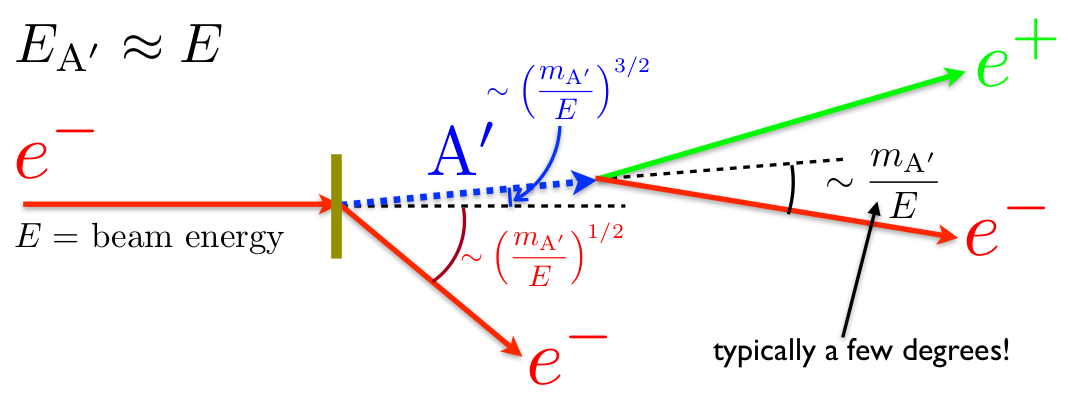
\includegraphics[width=0.85\textwidth]{figs/motivation/ap_kinematics.png}
    \caption{The kinematics for heavy photon ($\aprime$) produced from an electron on a fixed target. In general, $\aprime$s retain most of the incident beam energy, remain close to the beam axis due to a small recoil angle, and have a small opening angle.}
    \label{fig:kinematics}
\end{figure}

High luminosity fixed target experiments, that is experiments with a high intensity beam incident on a thin metal foil, can probe theoretically favored regions of the heavy photon parameter space. Production mechanisms are analogous to that of regular photon bremsstrahlung, called ``dark bremsstrahlung'', albeit, with suppressed rates due to the weak effective coupling of the $\aprime$ to electric charge and significantly different kinematics because of the relatively large mass of the $\aprime$ \cite{Tsai:1973py}. The kinematics of heavy photons can be calculated from the Weizacker-Williams Approximation (WWA) where the nucleus is replaced by an effective photon flux. This gives the production differential cross-section for an electron with energy $E_0$ incident on a fixed target as 

\begin{equation}
    \frac{\mathrm{d}\sigma}{\mathrm{d}x \mathrm{d} \ cos \theta_{\aprime}} \approx \frac{8Z^2 \alpha^3 \epsilon^2 E_0^2}{U^2} \frac{\chi}{Z^2} \left( 1-x+\frac{x^2}{2}-\frac{x(1-x)m^2_{\aprime}(E_0^2x\theta^2_{\aprime})}{U^2} 
    \right)
    \label{eqn:epsilon1}
\end{equation}

where $E_0$ is the beam energy, $x=E_{\aprime}/E_0$, $E_{\aprime}$ is the energy of the $\aprime$, and $\theta_{\aprime}$ is the angle from the beam in the lab frame \cite{Bjorken:2009mm} \cite{Beranek:2013yqa}. The value $\chi/Z^2$ is related to the electric form factor and is in the range $\sim 5-10$ for the HPS range of interest. The function $U(x,\theta_{\aprime})=E_0^2x\theta_{\aprime}^2+m_{\aprime}^2 \frac{1-x}{x}+m_e^2 x$ is related to the virtuality of the intermediate electron. The characteristic angle of emission is set by $U(x,\theta_{\aprime})-U(x,0) \sim U(x,0)$ which occurs at $\theta_{\aprime} \sim \frac{m_{\aprime} \sqrt{1-x}}{xE_0}$.

Integrating over angle $\theta_{\aprime}$ and neglecting the mass of the electron $m_e$ and assuming that $m_e \ll m_{\aprime} \ll E_0$ and $x\theta^2_{\aprime} \ll 1$, the differential cross-section becomes

\begin{equation}
    \frac{\mathrm{d}\sigma}{\mathrm{d}x} \approx \frac{8Z^2 \alpha^3 \epsilon^2 x}{m_{\aprime}^2} \frac{\chi}{Z^2} \left( 1+\frac{x^2}{3(1-x)} \right)
    \label{eqn:epsilon2}
\end{equation}

This equation reduces to the photon bremsstrahlung cross-section in the limit that $m_{\aprime} \rightarrow 0$. Since $U(x,0)$ is minimized, the $\aprime$ production rate is maximum at $x \approx 1$, showing that $\aprime$s take most of the incident electron's energy $E_{\aprime}\approx E_0$. There is also a cutoff value of $1-x$ at max$\left( \frac{m_e^2}{m^2_{\aprime}},\frac{m^2_{\aprime}}{E_0^2} \right)$ and a median of max$\left( \frac{m_e^2}{m^2_{\aprime}},\frac{m^2_{\aprime}}{E_0^2} \right)$. The $\aprime$ emission angle cutoff is given by max$\left( \frac{\sqrt{m_{\aprime}m_e}}{E_0},\frac{m_{\aprime}^{3/2}}{E_0^{3/2}} \right)$ and is much smaller than the opening angle of the decay products $\aprime \sim m_{\aprime}/E_0$. The recoil electron has a recoil angle of about $\theta_{R} \sim (\frac{m_{\aprime}}{E_0})^{1/2}$.

The overall $\aprime$ rate is proportional $\frac{\alpha^3 \epsilon^2}{m_{\aprime}^2}$, thus decreasing with increasing $\aprime$ mass, and is reduced from ordinary photon bremsstrahlung by a factor of $\frac{\epsilon^3 m_e^2}{m_{\aprime}^2}$. A typical decay length as measured in the lab frame $\gamma c\tau$ can be calculated from Eq. \ref{eqn:ctau}.

\begin{equation}
    \gamma c\tau=\frac{3\hbar E_0}{N_{eff}m_{\aprime}^2 \alpha \epsilon^2 c}
    \label{eqn:gammactau}
\end{equation}

%$\theta_{\aprime} \sim (\frac{m_{\aprime}}{E_0})^{3/2}$

%$\theta_{R} \sim (\frac{m_{\aprime}}{E_0})^{1/2}$

 For a fixed target experiment that attempts to reconstruct vertex positions, these kinematics provide significant challenges particularly from a highly boosted particle with a small opening angle. A schematic of the basic kinematics and $\aprime$ production from an electron incident on a fixed target is shown in Fig. \ref{fig:kinematics}.
 
 \clearpage
 
 \section{Fixed Target Backgrounds}\label{sec:backgrounds}
 
 \begin{figure}[!h]
    \centering
    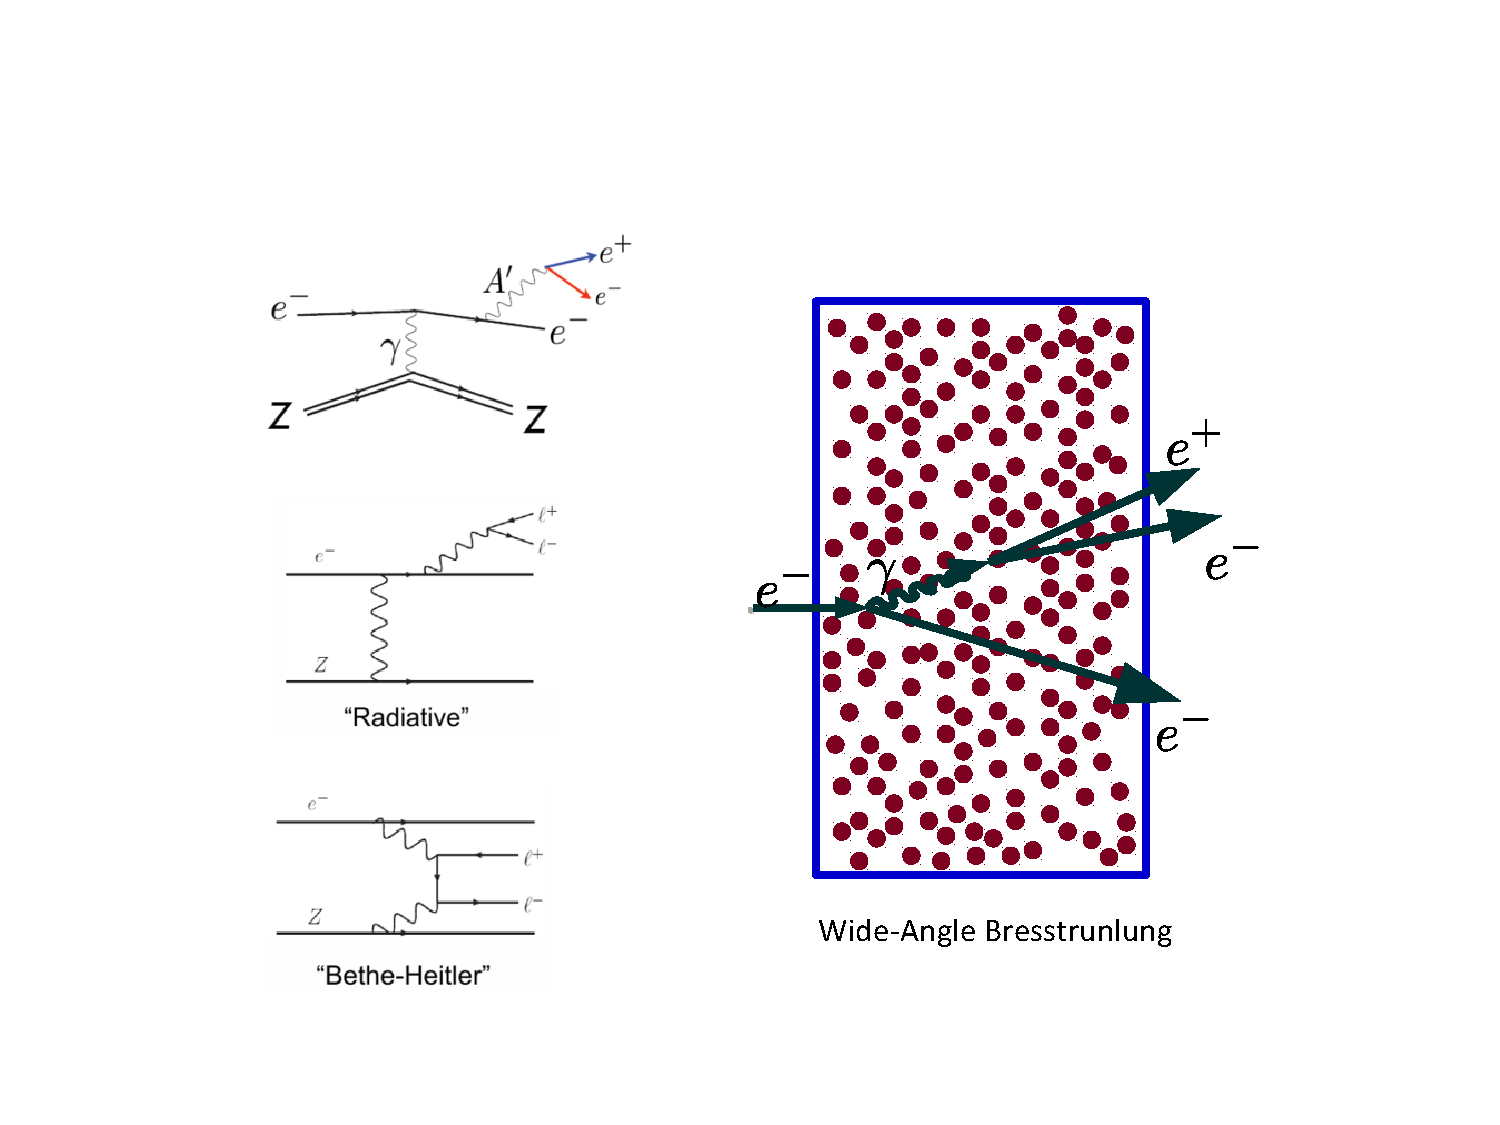
\includegraphics[width=1.\textwidth]{figs/recon/feynman-diagram.pdf}
    \caption{Left: Feynman diagrams for A$^{'}$ (top), RAD (middle) and BH (bottom) events. Right: A conversion of a WAB process.}
    \label{fig:feynman-diagram}
\end{figure}
 
 There are three main sources of physics backgrounds that are electro-produced in a fixed target that have an $\epem$ final state. The first two are prompt QED processes ($e^- Z \rightarrow \epem e^- Z$) called ``tridents'' because of the three-lepton final state. The other main $\epem$ background is bremsstrahlung production followed by pair conversion ($e^- Z \rightarrow e^- \gamma Z$ and then $\gamma Z \rightarrow \epem Z$) which can reconstruct as trident-like due to the three-lepton final state. These are not prompt since the conversion will occur from an on-shell $\gamma$ in either the target or any material in the detector. Their Feynman Diagrams are shown shown in Fig. \ref{fig:feynman-diagram}.
 
 The two types of trident processes are called ``radiatives'' and ``Bethe-Heitler'' tridents. Radiative tridents have identical kinematics to $\aprime$s. Because of this, radiative tridents constitute an irreducible prompt background that can only be distinguished from $\aprime$s through either a mass resonance in the $\epem$ invariant mass spectrum or through a finite decay length for sufficiently small $\epsilon^2$. However, the identical kinematics do provide a way to compute the expected $\aprime$ rates directly from counting $\epem$ pairs in the data and then using Eq. \ref{eqn:radiatives}.
 
 Bethe-Heitler diagrams, by itself, can be kinematically distinguished from the $\aprime$ and radiative diagrams and generally have softer daughter $\epem$ pairs ($\epem$ pair is not peaked at high $x$). This difference in kinematics is illustrated in Fig. \ref{fig:pvsp}. In addition, there are interference terms between radiative tridents and Bethe-Heitler tridents which make a significant contribution to the overall cross-section, but make it impossible to physically distinguish between recoil and daughter electrons where either particle paired with a positron is a potential background. However, even when selecting only $\epem$ pairs at high $x$ where radiative tridents peak, the Bethe-Heitler tridents and cross terms (altogether called ``non-radiative'' tridents) still dominate the rate of radiative tridents by nearly an order of magnitude.
 
 The last main background are known as wide-angle bremsstrahlung (WABs) where a photon and electron are both emitted from the target at large angles from the beam axis into the acceptance of HPS. The photon can either convert in the target or in a silicon plane in the tracker. There is a very large rate of WABs; however, only a small fraction are in HPS acceptance. The WABs that reconstruct a vertex with the daughter positron and the recoil electron are a background, though it will reconstruct at the primary even though the converted photon itself can be a displaced vertex. The rates of converted WABs with an $\epem$ pair in opposite halves of the detector after reconstruction is comparable to radiative tridents.
 
 \begin{figure}
    \centering
    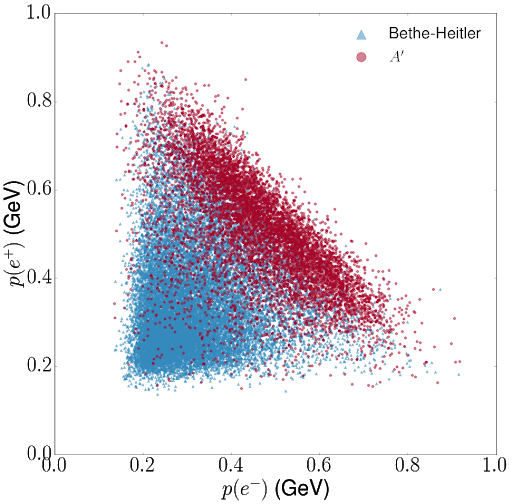
\includegraphics[width=0.5\textwidth]{figs/selection/p_vs_p.png}
    \caption{Positron momentum vs electron momentum comparing Bethe-Heitler tridents and $\aprime$s (and hence radiative tridents). $\aprime$s generally have a large $x$ in comparison to Bethe-Heitler. This is for a beam energy of 1.06 GeV.}
    \label{fig:pvsp}
\end{figure}

 

\section{Overview of HPS}\label{sec:hps}

The Heavy Photon Search (HPS) is a fixed target experiment at Jefferson Laboratory that searches for electro-produced heavy photons from a high energy electron beam and utilizes a compact forward acceptance spectrometer to capture the charged-lepton decay products of heavy photons and reconstruct their vertex positions and masses \cite{Battaglieri:2014hga}. The main components of HPS consists of a silicon vertex tracker (SVT) used for reconstruction of particle trajectories and an electromagnetic calorimeter (Ecal) used for timing and triggering. 

HPS searches for heavy photons using two distinct methods. The first method is a basic resonance search, or ``bump hunt'', where a search for a resonance in the invariant mass spectrum of $e^+e^-$ pairs at the heavy photon mass over a large background of QED processes is performed \cite{article}. HPS offers comparable sensitivity with other experiments that can perform a similar search and offers a relatively wide mass range over $e^-$ fixed-target competitors. However, HPS is not expected to probe new territory with the resonance search with the currently planned run time.

The second search method is a displaced vertex search where a secondary vertex displaced from the target is distinguished from a large prompt QED background \cite{adrian2018search}. The fact that HPS can search for long-lived heavy photons by actually reconstructing the vertex instead of using a much simpler beam dump experiment makes HPS uniquely able to probe a region of phase space of particles with short $c\tau$ values on the order of 1 - 10 mm.

In order to successfully perform these two searches, HPS must accomplish two difficult challenges. First, the heavy photon kinematics require large acceptance and excellent vertex resolution. This results in silicon from the first layer of the SVT to be 0.5 mm from an intense electron beam risking both highly non-linear radiation damage to the sensors and challenges of particle occupancy in the detector. The second challenge requires separating a large number of prompt QED processes on the order of $10^8$ that undergo multiple scattering in the tracker that may reconstruct downstream of the target from only a few true displaced vertices which are from a long-lived particles decaying beyond the tails of the prompt background distribution. The remainder of this thesis will focus on the methods and results from the displaced vertex search.

%Existence of DM \cite{Clowe:2006eq}

%Charmonium \cite{Gaiser:1982yw}

%Low energy frontier \cite{Jaeckel:2010ni}

%CP Conservation \cite{Peccei:1977hh}

%Annihilating DM \cite{Cholis:2008hb}

%Axions \cite{Tsai:1986tx}

%Boson Pair Production \cite{Kim:1973he}

%Axions \cite{riordan1987}

%Light Higgs Boson \cite{davier1989}